% LaTeX support: latex@mdpi.com
%  In case you need support, please attach all files that are necessary for compiling as well as the log file, and specify the details of your LaTeX setup (which operating system and LaTeX version / tools you are using).

% You need to save the "mdpi.cls" and "mdpi.bst" files into the same folder as this template file.

%=================================================================
\documentclass[information,article,submit,moreauthors,pdftex,10pt,a4paper]{Definitions/mdpi}

% If you would like to post an early version of this manuscript as a preprint, you may use preprint as the journal and change 'submit' to 'accept'. The document class line would be, e.g., \documentclass[preprints,article,accept,moreauthors,pdftex,10pt,a4paper]{mdpi}. This is especially recommended for submission to arXiv, where line numbers should be removed before posting. For preprints.org, the editorial staff will make this change immediately prior to posting.

%
%--------------------
% Class Options:
%--------------------
% journal
%----------
% Choose between the following MDPI journals:
% acoustics, actuators, addictions, admsci, aerospace, agriculture, agronomy, algorithms, animals, antibiotics, antibodies, antioxidants, applsci, arts, asi, atmosphere, atoms, axioms, batteries, bdcc, behavsci, beverages, bioengineering, biology, biomedicines, biomimetics, biomolecules, biosensors, brainsci, buildings, carbon, cancers, catalysts, cells, ceramics, challenges, chemengineering, chemosensors, children, cleantechnol, climate, clockssleep, cmd, coatings, colloids, computation, computers, condensedmatter, cosmetics, cryptography, crystals, cybersecurity, data, dentistry, designs, diagnostics, dairy, diseases, diversity, drones, econometrics, economies, education, electrochem, electrochemistry, electronics, energies, entropy, environments, epigenomes, est, fermentation, fibers, fire, fishes, fluids, foods, forecasting, forests, fractalfract, futureinternet, galaxies, games, gastrointestdisord, gels, genealogy, genes, geohazards, geosciences, geriatrics, hazardousmatters, healthcare, heritage, highthroughput, horticulturae, humanities, hydrology, informatics, information, infrastructures, inorganics, insects, instruments, ijerph, ijfs, ijms, ijgi, ijtpp, inventions, j, jcdd, jcm, jcs, jdb, jfb, jfmk, jimaging, jof, jintelligence, jlpea, jmmp, jmse, jpm, jrfm, jsan, land, languages, laws, life, literature, logistics, lubricants, machines, magnetochemistry, make, marinedrugs, materials, mathematics, mca, medsci, medicina, medicines, membranes, metabolites, metals, microarrays, micromachines, microorganisms, minerals, modelling, molbank, molecules, mps, mti, nanomaterials, ncrna, neonatalscreening, neuroglia, nitrogen, nutrients, ohbm, particles, pathogens, pharmaceuticals, pharmaceutics, pharmacy, philosophies, photonics, plants, plasma, polymers, polysaccharides, proceedings, processes, proteomes, publications, quaternary, qubs, reactions, recycling, religions, remotesensing, reports, resources, risks, robotics, safety, sci, scipharm, sensors, separations, sexes, sinusitis, smartcities, socsci, societies, soilsystems, sports, standards, stats, surfaces, surgeries, sustainability, symmetry, systems, technologies, toxics, toxins, tropicalmed, universe, urbansci, vaccines, vehicles, vetsci, vibration, viruses, vision, water, wem, wevj
%---------
% article
%---------
% The default type of manuscript is article, but can be replaced by:
% abstract, addendum, article, benchmark, book, bookreview, briefreport, casereport, changes, comment, commentary, communication, conceptpaper, correction, conferenceproceedings, conferencereport, expressionofconcern, extendedabstract, meetingreport, creative, datadescriptor, discussion, editorial, essay, erratum, hypothesis, interestingimages, letter, meetingreport, newbookreceived, opinion, obituary, projectreport, reply, reprint, retraction, review, perspective, protocol, shortnote, supfile, technicalnote, viewpoint
% supfile = supplementary materials
% protocol: If you are preparing a "Protocol" paper, please refer to http://www.mdpi.com/journal/mps/instructions for details on its expected structure and content.
%----------
% submit
%----------
% The class option "submit" will be changed to "accept" by the Editorial Office when the paper is accepted. This will only make changes to the frontpage (e.g., the logo of the journal will get visible), the headings, and the copyright information. Also, line numbering will be removed. Journal info and pagination for accepted papers will also be assigned by the Editorial Office.
%------------------
% moreauthors
%------------------
% If there is only one author the class option oneauthor should be used. Otherwise use the class option moreauthors.
%---------
% pdftex
%---------
% The option pdftex is for use with pdfLaTeX. If eps figures are used, remove the option pdftex and use LaTeX and dvi2pdf.

%=================================================================
\firstpage{1}
\makeatletter
\setcounter{page}{\@firstpage}
\makeatother
\pubvolume{xx}
\issuenum{1}
\articlenumber{5}
\pubyear{2019}
\copyrightyear{2019}
%\externaleditor{Academic Editor: name}
\history{Received: date; Accepted: date; Published: date}
%\updates{yes} % If there is an update available, un-comment this line

%% MDPI internal command: uncomment if new journal that already uses continuous page numbers
%\continuouspages{yes}

%------------------------------------------------------------------
% The following line should be uncommented if the LaTeX file is uploaded to arXiv.org
%\pdfoutput=1

%=================================================================
% Add packages and commands here. The following packages are loaded in our class file: fontenc, calc, indentfirst, fancyhdr, graphicx, lastpage, ifthen, lineno, float, amsmath, setspace, enumitem, mathpazo, booktabs, titlesec, etoolbox, amsthm, hyphenat, natbib, hyperref, footmisc, geometry, caption, url, mdframed, tabto, soul, multirow, microtype, tikz

\usepackage{caption}
\usepackage{subcaption}
\usepackage{todonotes}

%=================================================================
%% Please use the following mathematics environments: Theorem, Lemma, Corollary, Proposition, Characterization, Property, Problem, Example, ExamplesandDefinitions, Hypothesis, Remark, Definition
%% For proofs, please use the proof environment (the amsthm package is loaded by the MDPI class).

%=================================================================
% Full title of the paper (Capitalized)
\Title{Title}

% Authors, for the paper (add full first names)
\Author{Joseba Fernandez de Landa, Rodrigo Agerri* and I\~naki Alegria}

% Authors, for metadata in PDF
\AuthorNames{Joseba Fernandez de Landa, Rodrigo Agerri, I\~naki Alegria}

% Affiliations / Addresses (Add [1] after \address if there is only one affiliation.)
\address[1]{%
IXA NLP Group, University of the Basque Country UPV/EHU; e-mail@e-mail.com\\
%$^{2}$ \quad Affiliation 2; e-mail@e-mail.com
}

% Contact information of the corresponding author
\corres{Correspondence: e-mail@e-mail.com; Tel.: +x-xxx-xxx-xxxx}

% Current address and/or shared authorship
%\firstnote{Current address: Affiliation 3}
%\secondnote{These authors contributed equally to this work.}
% The commands \thirdnote{} till \eighthnote{} are available for further notes

%\simplesumm{} % Simple summary

% Abstract (Do not insert blank lines, i.e. \\)
\abstract{Social networks like Twitter are taking more and more importance nowadays, creating new ways of communication. They are also a useful tools for social and linguistic research, because there is a lot of public data available based on social interaction using such networks. The availability of this data is particularly important for less resourced languages, because it allows to apply current Natural Language Processing techniques to large amounts of unstructured data in order to analyze both the linguistic and social behavior of users based on the text they generate. In this work, the aim will be to study the linguistic and social aspects of young and adult people’s behavior based on their tweets’ contents and the social relations that can be structured from them. With this aim in mind, we have gathered over 6 million tweets written in Basque from more than 8000 users. First, we extracted and analyzed the crawled data to find the most popular topics. Then we classified each user’s tweet by age (young/adult) by establishing whether the writing style of each tweet is formal or informal. Several classification and topic modeling methods, both supervised and unsupervised, have been applied, offering each of them different insights with respect to the feasibility of the task with the available data. Second, we establish the relations that emerge between the users  based on their re-tweets, characterizing also the various communities that arise from the analysis of the data. We conclude that social research can be done using computer techniques, giving the opportunity both to segment communities based on demographic characteristics and to discover how they interact or relate to these, using large amounts of unstructured data.}

% Keywords
\keyword{Social Informatics; Social Networks; Basque language; Young people; Topics; Relations (list three to ten pertinent keywords specific to the article, yet reasonably common within the subject discipline.)}

% The fields PACS, MSC, and JEL may be left empty or commented out if not applicable
%\PACS{J0101}
%\MSC{}
%\JEL{}

%%%%%%%%%%%%%%%%%%%%%%%%%%%%%%%%%%%%%%%%%%
% Only for the journal Data:
%\dataset{DOI number or link to the deposited data set in cases where the data set is published or set to be published separately. If the data set is submitted and will be published as a supplement to this paper in the journal Data, this field will be filled by the editors of the journal. In this case, please make sure to submit the data set as a supplement when entering your manuscript into our manuscript editorial system.}

%\datasetlicense{license under which the data set is made available (CC0, CC-BY, CC-BY-SA, CC-BY-NC, etc.)}

%%%%%%%%%%%%%%%%%%%%%%%%%%%%%%%%%%%%%%%%%%
\begin{document}

%The order of the section titles is: Introduction, Materials and Methods, Results, Discussion, Conclusions for these journals: aerospace,algorithms,antibodies,antioxidants,atmosphere,axioms,biomedicines,carbon,crystals,designs,diagnostics,environments,fermentation,fluids,forests,fractalfract,informatics,information,inventions,jfmk,jrfm,lubricants,neonatalscreening,neuroglia,particles,pharmaceutics,polymers,processes,technologies,viruses,vision


\section{Introduction}\label{sec:introduction}

\indent Azken urteetan geroz eta ohikoagoak bilakatzen ari dira sare sozialak, gizakion bizitzaren zati geroz eta handiagoa hartzen ari baitira. Gure artean erlazionatzeko bide berriak ireki dira honi esker, oztopo espazial zein denboralak hautsi egin dira eta etengabeko konexioa ahalbidetu da komunitatearekin, nonahi eta noiznahi komunikatuta egoteko aukera irekiz \citep{castells2005sociedad}. Edonorekin, edozein momentutan, edozein tokitik konektatuta egoteko aukerak, harremantzeko modu hauen arrakastaren atzean daude, gazteen artean batez ere, eguneroko bizitzan normaltasunez txertatuz. Harremana oinarri duten kanal birtual hauek, ikerketarako aproposak diren informazio iturri berriak kontsideratu ditzakegu, gizarte ikerkuntzari ikerketa esparru berriak gehituz.\\
\indent Abagune berri honen aurrean, Eusko Ikaskuntza fundazioak, euskaraz hitz egiten duten gazteak nola harremantzen diren eta zertaz aritzen diren ezagutzeko asmoarekin, proiektu hau finantzatu du. Eusko Ikaskuntzak diruz lagundutako Master Amaierako Lan honetan, gazte euskaldunengana heltzeko modurik onena teknologia berrien bitartez dela erabaki da, aipatutako informazio iturri berriak irekiz eta ikerkuntza teknika aurreratuak erabiliz. Ikerketa honen metodo zein teknika berritzaileak aplikatzeko, beharrezkoa izan da IXA taldearen inplikazio zuzena, batez ere, masterraren bitartez trebetasunak eta ezagutza transmititzeko. Honekin, ikus daiteke Euskal Herriko testuinguruan aukerak badaudela erronka berriei aurre egiteko eta begi puntuan dauden gaiei lotzeko.\\
\indent Sare sozialetan euskal hiztun gazteek dauzkaten harreman sareen eta jorratzen dituzten gaien analisia egitea izan dira lan honen helburuak. Sare sozialak gazteon esparru bezala kontsideratu ditzakegu, haien sozializaziorako lanabes garrantzitsu bat izanik. Modu honetan, sareetan egiten den euskararen erabilera ezagutzea oso interesgarria da, garai berrietara moldatzeko euskarak daukan ahalmena ikusi, eta belaunaldi berrien espazioa diren sare sozialetan nola gauzatzen den ezagutzeko asmoz. Honela, euskararen egoera ezagutzetik gertuago egoteko aukera edukiko da, ikerketa-teknika tradizionalen osagarria izango den begirada berria eskainiz. Helburu horretarako Hizkuntzaren prozesamenduko tekniketan oinarritu gara, informatikako teknologiak gizarte-ikerkuntzan aplikatuz. Teknologia berrietan sortzen den edukia teknologia berrietan oinarritutako ikerketa-tekniken bitartez aztertuak izango dira, esparru berriak ikerketa-teknika berrien bidez ikertuz. Asmo horrekin, Twitter sare soziala hautatu da, identifikatutako euskal komunitate bat daukan sarea delako, eta baita, informazioa erauzterako orduan erraztasunak ematen dituelako ere, orokorrean jarioa publikoa delako, Instagram, Facebook eta Snapchat sareetan ez bezala.\\
\indent Honela, Twitter sare sozialean euskal komunitatearen inguruko ikerketa burutu da, sare sozialak informazio iturri garrantzitsu bat direla frogatuz. Era honetan, euskal txiolarien komunitatearen euskarazko 6 milioi txio baino gehiago lortu dira, ia 8000 erabiltzaile ezberdinetatik. Datu-base erraldoi honetatik (Big Data), interpretagarria den informazioa erauztea izango da asmoa, desegituratutako datu hauek ulergarri bihurtuz (Data Mining). Behin datuak erauzi direla, hurrengo pausua gazteak detektatzean oinarrituko da, adina bezalako ezaugarri demografikoak iradokitzeko saiakera eginez. Adinaren identifikazio automatikoaren bideragarritasun falta ikusita, hurbilpen bat egitea erabaki da, txioaren idazteko eran oinarritu gara erabiltzaile gazteak eta helduak ezberdintzeko hizkuntza ez-formalaren erabilera maiztasunean oinarrituz. Ezberdintze hau burutzea garrantzitsua da, gazteen errealitatea ezagutzea lehentasun bat baita lan honetan, bai gazteen eduki eta harremanak ezagutzeko, eta baita, ezkutuan dauden ezaugarri demografikoak antzemateko kapazitatea badagoela frogatzeko ere. Gazteak eta helduak sailkatzeko hurbilpena burututa egonda, bi izango dira ikerketa honetan argitu nahiko diren inkognitak, euskaldunek zertaz hitz egiten duten eta norekin harremantzen diren. Alde batetik, euskal txiolariek zein gairen inguruan hitz egiten duten ezagutzea izango da lehendabiziko asmoa, komunitate honen gairik errepikatuenak zeintzuk diren argituz. Honetarako, Hizkuntzaren prozesamenduko teknikak (NLP) erabiliko dira, testuetatik informazioa ateratzeko. Beste aldetik, euskal txiolariak nola harremantzen diren ezagutzea izango da bigarren asmoa, egindako birtxioetan oinarrituta, komunitateak zehaztu eta hauetako pertsona garrantzitsuak identifikatuz.\\
\indent Gizarte-zientzien eta konputazio-zientzien arteko konbinazioan kokatzen da lan honen ekarpen nagusia, aurrerapen teknologikoetan eta informazio mugagabean oinarritutako gizarte likidoa \citep{bauman2015modernidad} interpretatzen eta ulertzen lagunduko duen sinbiosia. Interneteko sareari esker, gizartea hobeto ulertzeko teknikak garatzeko orduan mugarri izan nahi du lan honek, gizarte-ikerkuntzan ireki den bide berri honetan lehenengo pausoak emanez. Lehenik eta behin, bilketan iraultza txiki bat piztea lortu da, interneteko datu-iturriak ustiatzeari esker, datu-iturri mugagabe bati ateak irekiz. Gizarte zientzietan datuak lortzea gutxi batzuen esku egon da beti suposatzen duen kostu altuagatik, baina Twitterren adibidez, Instagramen edo Facebooken ez bezala, edozeinek eskuratu ditzake datuak, informazioaren demokratizazio bat emanez. Hala ere, unibertsoa sare sozial zehatz honen erabiltzaileetara mugatzen da, iturri masiboagoak irekitzearen beharra dagoela azpimarratuz. Bigarrenik, datuen prozesaketan ere, hainbat teknika berritzaile aplikatzearen abantailak ikusi ahal izan dira. Zehatzago esanda, sare sozialetako erabiltzaile ezberdinen idatzizko adierazpen oinarrituta, zertaz hitz egiten duten eta nola harremandu diren antzematea lortu da. Honez gain, Ikasketa Automatikoan oinarritutako teknikei esker, ezaugarri demografikoak iradokitzeko ahalmena ere garatu da. Hau da, erabiltzaileen nolakotasunean oinarrituta, adina bezalako ezaugarri demografikoak intuitzeko kapaza den sistema bat garatu da. Honi esker, gizarte ikerlariontzat oinarrizkoak diren datuak (demografikoak kasu) igartzeko kapazitatea badagoela erakutsi da, datuak eskuragarri ez edukitzearen arazoa saihestuz. Hirugarrenik eta azkenik, datuen interpretagarritasuna errazteko asmoarekin, erabilitako teknikek bistaratze intuitibo eta grafiko bat izango dute, irudien laguntza izanik.



\section{Related Work}\label{sec:background}
%% Atal bakoitzaren artearen egoera azaldu beharko litzateke? edo orokorrean egindako lan guztiena?
General obs.

\subsection{Data Extraction}\label{sec:extraction_background}

Data extraction.

\subsection{Young/Adult Identification}\label{sec:identifier_background}

Analyzing demographic characteristics in social media is receiving increasing attention in the area of Social Media Mining.

Twitterren adinaren detekziorako
%, artearen egoerako metodo aipagarrienak bildu dira jarraian azaltzen zaigun taulan (\ref{tab:arte}. taula). %Taula horretan metodo bakoitzaren erreferentzia, sailkatzaile mota eta asmatze tasa ikusi daitezke. Taula %honetan ikusi daitekeen moduan,
sailkatzaile ohikoenak ataza honetarako \textit{Logistic Regression} \citep{nguyen2013old,morgan2017predicting} eta \textit{Support Vector Machine} \citep{rao2010classifying,al2012homophily,marquardt2014age} dira. Sailkatzaile guzti horiek ikasketa automatikoan oinarritutako metodo gainbegiratuak dira, guztiak tamaina esanguratsu bateko etiketatutako corpus batean oinarrituta. Ikerketa guzti horietan datuen etiketatzea erabiltzaile bakoitzaren adinean oinarrituta dago, eskuz erabiltzaile kopuru esanguratsu bat anotatu dutelarik.

%\begin{table}[H]
%  \centering
%  \begin{tabular}{|l|l|r|}
%    \hline
%    \textbf{Sistema} & \textbf{Sailkatzailea} & \textbf{Asmatze tasa}\\ \hline
%    Rao et al. (2010) & \textit{Support Vector Machine} & \% 74,11\\ \hline
%    Al Zamal et al.  (2012) & \textit{Support Vector Machine} & \% 80,50\\ \hline
%    Marquart et al. (2014) & \textit{Support Vector Machine} & \% 48,31\\ \hline
%    Nguyen et al. (2014) & \textit{Logistic Regression} & \% 86,32\\ \hline
%    Morgan-Lopez et al. (2017) & \textit{Logistic Regression} & \% 74,00\\ \hline
%  \end{tabular}
%  \caption{Bibliografiako sistemak, adinaren detekzioa Twitterren.}
%  \label{tab:arte}
%\end{table}

Jarraian sistema bakoitzean murgilketa txiki bat egingo da, etiketatutako corpusa eta klase kopurua ezagutzeko asmoarekin (\ref{tab:arte ezaug}. taula). Sistemak oso ezberdinak dira ikusi daitekeen moduan, behar ezberdinetara egokitutako ikerketak baitira. Alde batetik, eskuz etiketatutako corpus hauen tamaina ikerketaren arabera aldatuz doa, baina guztiek 300 eta 3000 erabiltzaile artean dauzkate etiketatuta. Bestalde, bibliografiako sistema onenek, beren sailkapena burutzeko asmoarekin, adin tarte bitarrak \citep{rao2010classifying,al2012homophily} edo hirutarrak \citep{nguyen2013old,morgan2017predicting} erabili dituzte, geroz eta klase gutxiago edukiz (bitarra edo hirutarra) sailkatzeko ataza errazago burutzen dela frogatuz.

Erabiltzaile bakoitza adinaren arabera sailkatzeko asmoz, lortutako txio bakoitzeko testua zein meta-datuak bezalako aldagaiak erabili dira. Honela, artearen egoerako autore ezberdinek, bakoitzak bere ezaugarri propioak aukeratu ditu, txioen testuaz gain, erabiltzaile zehatzen meta-datuetan oinarritutako hainbat ezaugarri ere konbinatuz. Hala ere, sistema hauek bata bestearengandik oso ezberdinak direla ikusi den arren, guztiek testua hartzen dute kontutan, gehienak sailkatzailea txioen idazkera estiloan oinarritzen direlarik \citep{rao2010classifying,al2012homophily,nguyen2013old,morgan2017predicting}.\\

\begin{table}[H]
  \centering
  \begin{tabular}{|l|l|c|r|}
    \hline
    \textbf{Sistema} & \textbf{Corpus tamaina} & \textbf{Klase kopurua} & \textbf{Hizkuntza}\\ \hline
    Rao et al.(2010) & 1000 erabiltzaile & 2 & Ingelera\\ \hline
    Al Zamal et al.(2012) & 400 erabiltzaile & 2 & Ingelera\\ \hline
    Marquart et al.(2014) & 306 erabiltzaile & 5 & Gaztelera\\ \hline
    Nguyen et al.(2014) & 3110 erabiltzaile & 3 & Nederlandera\\ \hline
    Morgan-Lopez et al.(2017) & 3184 erabiltzaile & 3 & Ingelera\\ \hline
  \end{tabular}
  \caption{Bibliografiako sistemak, adinaren detekzioa Twitterren.}
  \label{tab:arte ezaug}
\end{table}

Amaitzeko, esan beharra dago sailkatzaile bakoitzaren asmatze tasari (\textit{accuracy}) erreparatuz gero, oraindik bide luze bat geratzen dela adina bezalako ezaugarri demografikoak egoki iragartzeko sare sozialetan. Adinaren sailkatzaileen asmatze ahalmena perfekziotik urruti daudela kontutan hartuta, ikerketa soziala zaildu egiten da, oinarrizkoak diren datu demografikoetan errore altuak daudelako. Adina bezalako datuk gizarte ikerketaren oinarrietako bat dira eta errore altuak emaitzak desitxuratu ditzake. Hala ere, ezin dugu ahaztu, txikia baldin bada ere, errorea beti egongo dela, gizartea konplexutasunez beteta baitago eta orokortze perfektu bat izatea ezinezkoa izango litzateke. Horregatik, errorea izanda ere, gizarte multzo zehatz honen orokortasunak jasotzeko arazorik ez da egongo, euskal txiolari gazteen eta helduen arteko konparaketa orokor bat egitea baita asmoa.\\

\subsection{Topics}\label{sec:topics_background}

Extracting information from huge amounts of unstructured text is the aim of topic modeling. In this way, different approaches try to extract the common information that contains the numerous tweets scattered through the network, such as extract the topics covered by the event and the tweets \citep{hu2012lda}, real-time classification of twitter trends \citep{zubiaga2015real} or to compare the content of Twitter with a traditional news medium \citep{zhao2011comparing}. Apart from the different uses, they have to take into account the nature of the tweets because the length of the text makes the topic modeling have to be applied in a certain way, appropriate for short texts \citep{hong2010empirical}.

\subsection{Relations}\label{sec:connections_background}

There are several studies that have tried to identify different communities based on retweets. Among these, one can find studies about political polarization \citep{conover2011political}, political affiliation detection \citep{pennacchiotti2011democrats} or even studies about identifying communities in movements for independence \citep{zubiaga2017stance}. In these studies, based on the retweets made by the user, it shows that there is the possibility of identifying communities or groups. Therefore, in this specific work, similar methodologies will be used to predict how communities are formed and how they are related.


\section{Methodology}\label{sec:methodology}

To investigate the reality of young Basque Twitter users, the study is going to be divided into four different steps. The first step consist on identifying Basque Twitter users and extracting the data from this Social Network. After that, as second step, Basque Twitter users have been classified between adult and young users, based on the stile of the written tweet. Once basque Twitter users are separated between young and adults, we will try to find out the topics and relations of each of the groups. To find out the topics of these communities, we will take into account the personal tweets in basque of each user. On the other hand, to find out the relations, we will take into account the retweets in basque of each user. For each task indicated, a specific methodology will be used, as will be demonstrated below.

\paragraph{Data Extraction}

The first step consists on defining the social universe to investigate. The social universe is defined as all Twitter users who write in basque. With the purpose of identifying those basque writers in the whole Twitter network, a shortcut will be used, the list of Umap.eus\footnote{\url{https://umap.eus/}}. Once we know which users data extract, tweepy \citep{roesslein2009tweepy} package from Python will be used. Thanks to this package it will be possible to extract all the necessary information from each basque Twitter user.

\paragraph{Young/Adult Identifier}

The aim of this section is identifying young basque users, differentiating young users from the adult ones. This classification will not be made according to age, but based on the content of the messages, by which the text of personal tweets will be taken as a reference. Based on the text of the tweets, each tweet of a user is classified as formal or informal, depending on the writing style. When the concentration of informal tweets is high, it will be considered a young user, since young people have a more informal style \citep{nguyen2013old}. For that purpose, a small corpus has been labeled, labeling manually over 1,000 tweets as informal or formal. Three different methods have been used to train the classifier that will distinguish between formal and informal tweets, a non-supervised statistical model, machine learning and IXA pipes document classifier.

\paragraph{Topics}

On the one hand, for identifying the topics which basque users speak of, personal tweets in Basque language have been used. To do this, the Topic-Modeling technique is used, applying the LDA algorithm for that purpose. Specifically, gensim \citep{rehurek2010software} package has been used for applying LDA, so LDA can be applied to the obtained text from tweets. For an intuitive display, the \textit{LDAvis} method \citep{sievert2014ldavis} is used. This method publishes results as images, which helps interpreting the results.

\paragraph{Connections}

On the other hand, to know what the way of relating of the users is, retweets will be used. For that purpose, a graph based on the retweets will be used, the nodes being the users and each edges a retweet. For the creation of the graph the Ghepi program \citep{bastian2009gephi} has been used. Apart from that, modularity \citep{blondel2008fast} has been used to identify the subgroups of the graph that would represent different communities.


% #########################################################
% ################     DATA EXTRACTION     ################
% #########################################################
% Euskal txiolarietaz gain ere, modu orokorrago batean azaldu ataza (abstrakzio malia altuagoa) -->> hiztun gutxituen komunitateari buruzko analisia.

\section{Data Extraction}\label{sec:data-extraction}

As the first step the community we have to focus on has to be specified, in order to start extracting data from somewhere. With the intention of investigating a specific community, it is necessary to identify this community in the whole network, specifying the universe to be studied. In this case, people who publish tweets in Basque will be the community to investigate. For identifying basque speakers in Twitter, a list already prepared by Umap.eus has been used. This website includes in the list users who publish at least 20\% of their tweets in Basque\footnote{\url{https://umap.eus/}}. In this way, a list of 8,189 Basque users has been obtained, which will consist the sample for the investigation.

Once the community to investigate is specified and the sample of users, whom information is going to be gathered, is chosen, the data extraction will began. To extract the data from Twitter, \textit{tweepy} package from Python is used, choosing the \textit{timeline extraction} mode to gather the last 3,200 available tweets of each user of the sample. The data collection was performed between May 30 and 31, 2018, gathering more than 10 million tweets from 7,980 basque Twitter users (the Large Corpus). As the purpose of this investigation is to identify the content in Basque language of this users, the tweets generated are classified by language using metadata stored in the tweet. Once the content in basque is selected, personal tweets and retweets are separated, using each one for a specific task. After the classification, the characteristics of the Heldugazte corpus can be seen in the table \ref{tab:useful-data}\footnote{The dataset is publicly available at \url{https://github.com/ixa-ehu/heldugazte-corpus}.}.

\begin{table}[H]
  \centering
  \begin{tabular}{lll} \hline
     & \textbf{Personal tweets in Basque} & \textbf{Retweets in Basque}\\ \hline \hline
    \textbf{Tweets} & 3,171,785 & 2,891,136 \\
    \textbf{Terms} & 1,434,050 & 813,833 \\
    \textbf{Tokens}  & 37,350,268 & 39,329,204 \\ \hline
  \end{tabular}
  \caption{Characteristics of the Heldugazte corpus.}
  \label{tab:useful-data}
\end{table}

\section{Classifying Young/Adult Users}\label{sec:class-young-users}

In this section we present our work to classify Basque Twitter users as young or adult by analyzing their tweets' writing style. As we have seen in Section \ref{sec:identifier_background}, previous work includes automatic approaches to characterize users in the context of social networks and media, the most common being those related with genre and age \citep{cesare2017detection}. Our objective of developing a classifier to characterizing Basque Twitter users according to two stages of life (young/adult) is therefore placed within that research line.

Furthermore, section \ref{sec:identifier_background} also shows that most of previous work addresses the problem of classifying age stages using supervised machine learning techniques. This implies that some training data must be annotated according to the age or age stage of each user. Moreover state of the art  results indicate that classifying by age stages allows to obtain better results than when the problem is formulated in terms of age ranges \citep{nguyen2013old}. This seems to be due to the fact that shared experiences are easier to relate along time by using age stages rather than age ranges \citep{nguyen2016computational,eckert2017age}. Therefore, in this work we decided to focus on classifying users in terms of two general age stages, namely, young and adult.

However, this decision encountered an early methodological problem. In order to annotate tweets written in Basque according to the age stages of their authors it is obviously necessary to have available some data providing such information. Unfortunately, for the large majority of users from which we mined tweets this information is not available. Thus, our decision to overcome this problem consisted of focusing on the information available on the tweets themselves by taking into account writing style features. After all, most of the previous work widely uses writing style based features in order to classify users in terms of age stages \citep{rao2010classifying,al2012homophily,nguyen2013old,morgan2017predicting}.

It has been suggested that adults tend to use more conventional language \cite{nguyen2013old} whereas for young people it is more common to display repetitions and out of dictionary words \citep{rao2010classifying,rosenthal2011age,morgan2017predicting}. Generalizing on this idea we will assume that writing style changes according to the age of the twitter user. In other words, we will consider that \emph{adult writing style} is more formal whereas young people's style can be seen as more informal. Therefore, we will be classifying users as young/adult by classifying their tweets in terms of formal or informal language.

\subsection{Experimental Framework}\label{sec:exper-fram}

Following the setting established above, we will address the problem of classifying each tweet as \emph{formal} or \emph{informal} by means of several machine learning approaches. First, we will apply one unsupervised statistical method based on perplexity \cite{gamallo2017language}. Second, we will experiment with several supervised approaches: (i) a baseline method using sparse, \emph{one-hot} word representations \cite{pedregosa2011scikit}; (ii) a feature-based method using word representations as continuous word vectors, namely, word embeddings  on top of the baseline developed in (i) \cite{mikolov2013distributed,pennington-etal-2014-glove,mikolov-etal-2018-advances}; (iii) an off-the-shelf system which uses clustering features for representing the documents \cite{agerri2016robust,agerri2019language} and (iv), a deep learning approach leveraging character contextual word embeddings and a neural network architecture \cite{akbik2018contextual}.

We will develop a classifier with each of the methods listed above and evaluate it on a held-out, gold-standard dataset manually annotated at tweet level for the categories of \emph{formal} and \emph{informal}. The method that obtains the best results in the experiments will be then used to annotate the 6 million tweets obtained thereby classifying their authors as \emph{young} or \emph{adult}. In this sense, users will be classified according to the writing style of the tweets in their timelines.

In the rest of this section we will describe the process of manual annotation of the training and evaluation data. After that, we describe the configuration settings of each of the systems used or implemented for the experiments.

\subsubsection{Gold Standard Data}\label{sec:gold-standard-data}

\begin{table}[H]
  \centering
  \begin{tabular}{lr} \hline \hline
    Total number of tweets & 1.000 \\
    Formal & 492 \\
    Informal & 508 \\
    Tokens in shortest tweet & 5 \\
    Tokens in longest tweet & 34 \\
    Token avg. & 9.66 \\ \hline
  \end{tabular}
  \caption{Gold standard corpus.}
  \label{tab:gold-corpus}
\end{table}

In order to focus on learning to classify tweets according to writing style, we decided to clean the tweets keeping only those words that contained alphanumeric characters. Thus, we removed emoticons, hashtags, users' names (@) and URL links. Furthermore, we only considered those tweets that contained more than 4 tokens. We then randomly selected 1000 tweets sent from personal accounts from the 6 million tweet dataset collected as described in Section \ref{sec:data-extraction}. One annotator manually labeled every tweet as \emph{formal} or \emph{informal}. To manually label the tweets, a qualitative methodology was followed: all those tweets that contained out of vocabulary words or colloquial expressions were classified as informal. This methodology has been motivated by previous work on classifying formal and colloquial tweets \cite{gonzalez2015analysis}. Table \ref{tab:gold-corpus} shows the main features of our manually annotated dataset. For the experiments described in the next four subsections, we split the gold standard corpus in three sets, leaving 65\% for training and \%35 for testing.

\subsubsection{Unsupervised approach: \textit{Perplexity}}\label{sec:unsup-appr-text}

Perplexity is a widely-used evaluation metric for language models built with n-grams extracted from text corpora \cite{chen1999empirical}. Furthermore, it has been used for specific tasks, namely, to classify between formal and colloquial tweets \cite{gonzalez2015analysis} or for language identification between similar languages \cite{gamallo2017language}. Both works inspire our approach to classifying tweets as formal or informal using perplexity. The former showed that perplexity could be useful to indirectly detect out-of-vocabulary words in tweets \cite{gonzalez2015analysis}. More importantly for us, the latter formally proposed the concept of \emph{perplexity-based distance} between two languages.

A perplexity-based distance between two languages is established by ``comparing the n-grams of a text in one language with the n-gram language model trained for the other language. Then, the perplexity of a test text T in language L2, given the language model LM of language L1, can be used to define the distance, between L1 and L2'' \cite{gamallo2017language}. According to this definition, low perplexity indicates close proximity between languages L2 and L1.

In order to classify tweets as \emph{formal} or \emph{informal}, we will calculate the perplexity-based distance between a tweet with respect to a character-based 7-gram language model. If the perplexity-based distance between each tweet and the character-based n-gram language model is low, then we will classify it as \emph{formal} and \emph{vice versa}. Of course, for this approach to work we need to establish a threshold so that if the perplexity-based distance is lower than the threshold the tweet is labeled as \emph{formal} and if higher, as \emph{informal}.

Our method to calculate such threshold proceeds in the following manner. First, we build a 7-gram character-based language model using the data from a corpus composed of texts from the Basque  Egunkaria and Berria newspapers. Second, we take the tweets in the training set (65\% of the dataset) and classify each of them according to the perplexity-based distance with respect to the language model. We tried every value in the [0,10] range
with an increment of 0.1 as threshold. Third, we computed precision, recall and accuracy comparing the prediction of the threshold according to the perplexity value with respect to the gold-standard labels in the training data. Finally, the threshold chosen will be the value in which all the three metrics converge. As shown by Figure \ref{fig:threshold}, we found out that the best threshold value was around 4.4. We will use this value in order to evaluate this approach in Section \ref{sec:experimental-results}.

\begin{figure}[H]
  \centering
  \begin{subfigure}[b]{0.48\linewidth}
    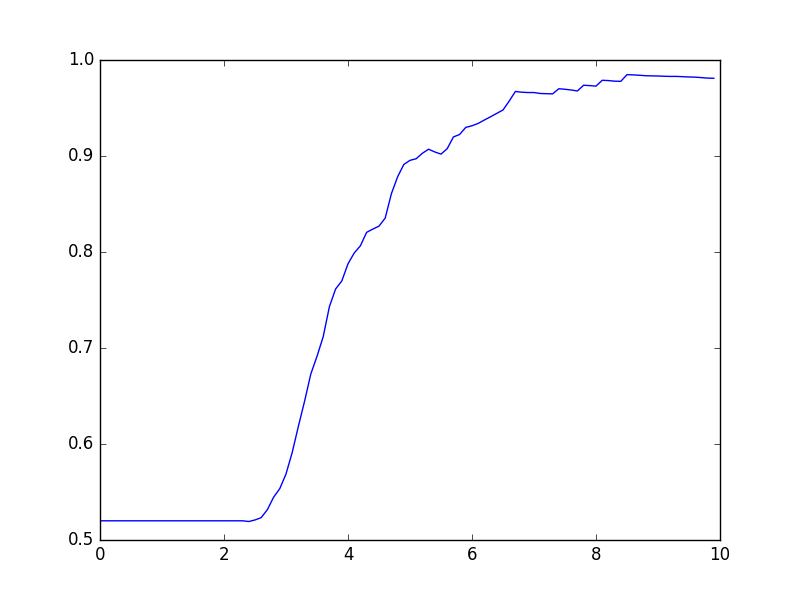
\includegraphics[width=\linewidth]{precision}
    \caption{Precision.}\label{fig:precision}
  \end{subfigure}
  \begin{subfigure}[b]{0.48\linewidth}
    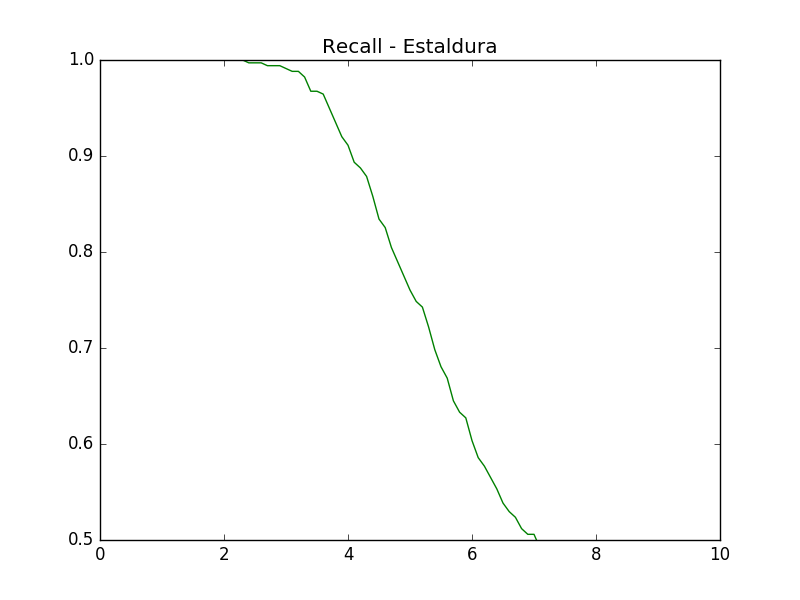
\includegraphics[width=\linewidth]{recall}
    \caption{Recall.}\label{fig:recall}
  \end{subfigure}
  \begin{subfigure}[b]{0.48\linewidth}
    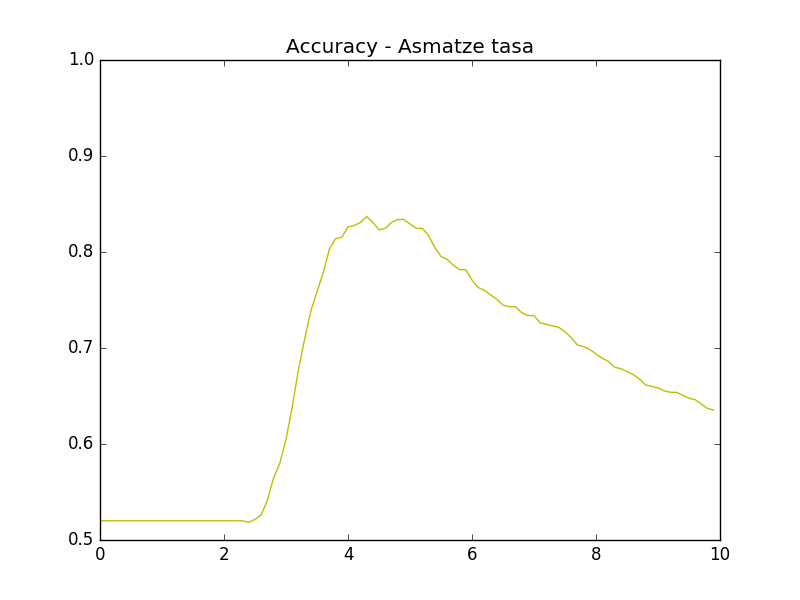
\includegraphics[width=\linewidth]{accuracy}
    \caption{Accuracy.}\label{fig:acc}
  \end{subfigure}
  \begin{subfigure}[b]{0.48\linewidth}
    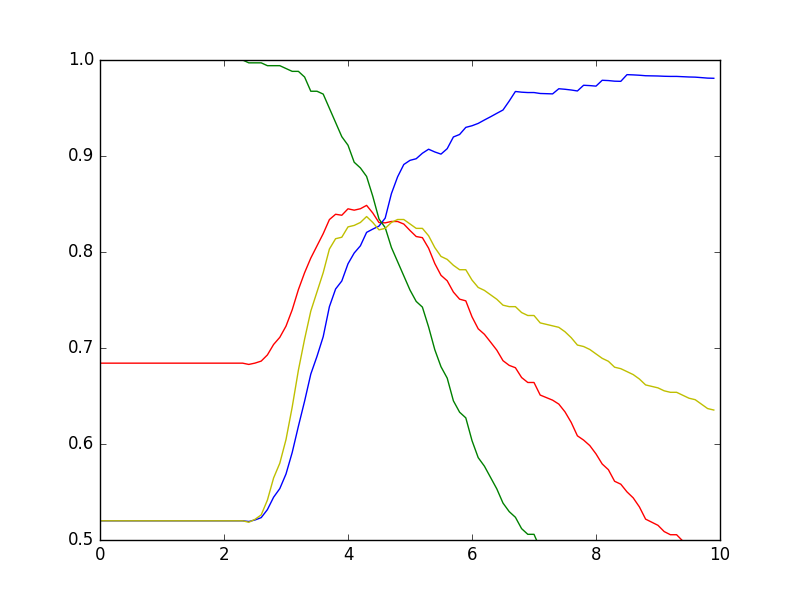
\includegraphics[width=\linewidth]{denaperp}
    \caption{Optimal threshold value on the training data.}\label{fig:threshold}
  \end{subfigure}
\end{figure}

Table \ref{tab:perplexitytrain} displays the results of classifying the tweets in the training data using perplexity-based distance using the value 4.4 as threshold. The obtained overall accuracy using 4.4 as threshold was 0.831.

\begin{table}[H]
  \centering
  \begin{tabular}{lcccc} \hline
    Label & Error & Precision & Recall & F1 \\ \hline \hline
    Informal & 48 & 0.824  & 0.858  & 0.841 \\
    Formal & 62 & 0.839 & 0.801 & 0.820 \\ \hline
  \end{tabular}
  \caption{Results of the unsupervised approach on the training set.}
  \label{tab:perplexitytrain}
\end{table}

\subsubsection{Supervised Baseline}\label{sec:sparse-word-repr}

The first baseline applying supervised machine learning will be done to test various learning algorithms using the gold standard dataset described in Section \ref{sec:gold-standard-data}. More specifically, we will be simply applying a bag of words representation which represents each document (tweet) according to the word frequencies in each document. The result is a very sparse word representation where the dimension of the vector representing each word is equal to the number of words in the corpus. In this setting, we apply six of the most common machine learning algorithms with default parameters using the scikit-learn library \cite{pedregosa2011scikit}. Table \ref{tab:acc-ml} reports their performance by means of 5-fold cross validation on the training data.

\begin{table}[H]
  \centering
  \begin{tabular}{lr} \hline
    Machine Learning Classifier (BoW) & Accuracy \\ \hline \hline
    5-NN (k-NN) &  0.614 \\
    Decision Tree &  0.677 \\
    Random Forest &  0.707 \\
    Naive Bayes & 0.765 \\
    Logistic Regression & 0.775 \\
    \textbf{SVM} & \textbf{0.777} \\ \hline
  \end{tabular}
  \caption{Bag of words results via 5-fold cross-validation on the training set.}
  \label{tab:acc-ml}
\end{table}

As it can be seen, the best performing algorithms in this baseline setting are Logistic Regression and SVM. This is not surprising given the ability of SVM to perform well with very few labeled data. Next, we decided to experiment with a less-sparse representation of the tweets by means of pre-trained word embeddings and the SVM classifier.

\subsubsection{Pre-trained Word Embeddings}\label{sec:pre-trained-word}

Distributed word representations or word embeddings are widely used nowadays in Natural Language Processing. Several techniques have been proposed in order to obtain word embeddings, most of them based on the hypothesis that the meaning of a word is defined by the context in which it appears \cite{mikolov2013distributed,pennington-etal-2014-glove}. Thus, obtaining word embeddings usually requires large quantities of good quality training data which makes it difficult when experimenting with less-resourced languages such as Basque. However, FastText provides pre-trained models for many languages, including Basque \cite{mikolov-etal-2018-advances} by using the common crawl data\footnote{\url{http://commoncrawl.org}}. The Basque model they distribute is trained on both Common Crawl and Wikipedia using CBOW with position-weights, in 300 dimension, with character n-grams of length 5, a window of size 5 and 10 negatives\footnote{\url{https://fasttext.cc}}.

For this experiment, we map the words in the corpus to their real vector representation in the FastText model and average all the vectors with respect to the vocabulary. We optimize the C hyperparameter using accuracy and evaluate by 5-fold cross-validation on the training data. Table \ref{tab:svmf1} reports the detailed results of the 5-fold cross-validation using C$=1.1$ as hyperparameter.

\begin{table}[H]
  \centering
  \begin{tabular}{lcccc}
    \hline
    Label & Error & Precision & Recall & F1 \\ \hline \hline
    Informal & &  &   &  \\
    Formal &  &  &  &  \\ \hline
  \end{tabular}
  \caption{SVM (rbf and FastText embeddings) results via 5-fold cross-validation on the training set.}
  \label{tab:svmf1}
\end{table}

\subsubsection{IXA pipes}\label{sec:ixa}

The document classification system included in the IXA pipes tools, \emph{ixa-pipe-doc}, aims to establish a simple and shallow feature set, avoiding any linguistic motivated features, with the objective of removing any reliance on costly extra gold annotations and/or cascading errors if automatic annotations are used. The underlying motivation is to obtain robust models to facilitate the development of document classification systems for several languages, datasets and domains while obtaining state of the art results.

\emph{ixa-pipe-doc}, as a component of IXA pipes, includes a simple method to combine various types of clustering features induced over different data sources or corpora. This method has already obtained state of the art results in several tasks such as newswire Named Entity Recognition \cite{agerri2016robust} and Opinion Target Extraction \cite{agerri2019language}, both in out-of-domain and in-domain evaluations and for several languages, including Basque.

The system consists of: (i) Local, shallow features based mostly on orthographic, word shape and n-gram features plus their context; (ii) three types of simple clustering features, based on unigram matching; (iii) publicly available gazetteers, such as sentiment lexicons. Specifically, \emph{ixa-pipe-doc} implements, on top of the local features, a combination of word representation features: (i) Brown \cite{brown1992class} clusters, taking the 4th, 8th, 12th and 20th node in the path; (ii) Clark \cite{clark2003combining} clusters and, (iii) Word2vec \cite{mikolov2013distributed} clusters, based on K-means applied over the extracted word vectors using the skip-gram algorithm. The implementation of the clustering features looks for the cluster class of the incoming token in one or more of the clustering lexicons induced following the three methods listed above. If found, then we add the class as feature. The Brown clusters only apply to the token related features, which are duplicated\footnote{More details, including examples of the features are provided in Agerri and Rigau \cite{agerri2016robust,agerri2019language}.}.

Clusters of words provide denser document representations. Although still a one-hot vector representation, the dimensions of the representation gets reduced to the number of clustering classes used. This is done by mapping the words in the document to the words in each of the clustering lexicons \cite{turian-ratinov-bengio:2010:ACL}. To avoid duplication of efforts, the system uses the Apache OpenNLP project implementation of Maxent \footnote{\url{http://opennlp.apache.org/}} customized with the features described above.

For the experiments, we used pre-trained clusters using the Elhuyar Web Corpus \cite{leturia2012evaluating} and from a 600M word corpus obtained from crawling local news sites (Local News Corpus). The number of clusters trained with each algorithm and data source was the following: 100-800 clusters using the Clark and Word2vec methods, and 1000, 2000 and 3200 classes with the Brown algorithm. The best combination of features was obtained by performing every possible permutation between them in a 5-fold cross validation setting using the gold standard training data. Following this methodology, the best configuration consisted of the features listed in Table \ref{tab:clusters} (we did not use any local or lexicon-based features, just the clustering representations).

\begin{table}[H]
  \centering
  \begin{tabular}{l|l} \hline
    Cluster type & Corpus - \# clusters\\ \hline \hline
    Brown & EWC-3200 \\
    Clark & EWC-600 \& LNC-300  \\
    Word2vec & EWC-300 \& LNC-500\\ \hline
  \end{tabular}
  \caption{Source data and number of clusters used with ixa-pipe-doc system. EWC: Elhuyar Web Corpus. LNC: Local News Corpus.}
  \label{tab:clusters}
\end{table}


Table \ref{tab:ixa-ml-garapen} provides the results per class using \emph{ixa-pipe-doc}. As it can be seen, they are the best results obtained so far both in terms of accuracy (0.887) and F1 measure.

\begin{table}[H]
  \centering
  \begin{tabular}{lcccc}
    \hline
    Label & Error & Precision & Recall & F1\\ \hline \hline
    Informal & 32 & 0.892  & 0.886  & 0.889 \\
    Formal & 30 & 0.883 & 0.889 & 0.886 \\ \hline
  \end{tabular}
  \caption{ixa-pipe-doc results via 5-fold cross-validation on the training set.}
  \label{tab:ixa-ml-garapen}
\end{table}


\subsubsection{Flair}\label{sec:neural-architecture}

Flair refers to both a deep learning toolkit based on neural networks and to a specific type of character-based contextual word embeddings \cite{akbik2018contextual}. Unlike static word embeddings such as those of Word2vec \cite{mikolov2013distributed}, Glove \cite{pennington-etal-2014-glove} or FastText \cite{mikolov-etal-2018-advances}, contextual embeddings allow to obtain word representations in a vector space taking into account the sense of the word given the context in which it appears. Thus, while a polysemous word would be given a unique real valued representation in the FastText pre-trained word embedding model used in Section \ref{sec:pre-trained-word}, Flair embeddings will aim to provide different representations depending on the contextual meaning of the word. Another important difference is that Flair embeddings are not word-based, they are trained by modeling words as sequences of characters.

Flair embeddings have been successfully applied to sequence labelling tasks obtaining best results for a number of public benchmarks \cite{akbik2018contextual}. In this paper, we apply the Flair toolkit to train document classification systems for classifying tweets as \emph{formal} or \emph{informal}. Flair provides a recurrent neural network (RNN) architecture (Cho et al., 2014) to represent documents, modelling text as a sequence of characters passed to the RNN which at each point in the sequence is trained to predict the next character \cite{akbik2018contextual}. We used this architecture to train document classification systems leveraging several pre-trained word embedding models: Flair contextual embeddings for Basque, character embeddings and the FastText Basque embeddings used previously. The Flair contextual embeddings for Basque were trained on various sources and it contains around 249M words. We performed 5-fold cross-validation on the training data obtaining the best results with a combination of the Flair and the FastText embeddings, obtaining 0.808 in word accuracy. Table \ref{tab:flair} reports on the final cross-validation results for each label.

\begin{table}[H]
  \centering
  \begin{tabular}{lcccc}
    \hline
    Label & Error & Precision & Recall & F1 \\ \hline \hline
    Informal & 61 & 0.898 & 0.759  & 0.823 \\
    Formal & 65 & 0.730 & 0.878 & 0.792 \\ \hline
  \end{tabular}
  \caption{Flair results via 5-fold cross-validation on the training set.}
  \label{tab:flair}
\end{table}


\subsection{Experimental Results}\label{sec:experimental-results}

In order to finish our experiments, we evaluated the approaches that obtained best cross-validation results on the gold standard test set. We chose to compare the best systems: the SVM model with FastText word embeddings, the perplexity-based distance method, ixa-pipe-doc and Flair. Table \ref{tab:testresults} reports the final results of our experiments to obtain a good classifier of Basque tweets according to writing style (formal/informal).

\begin{table}[H]
  \centering
  \begin{tabular}{lcccccc} \hline
    System & Accuracy & Label & Error & Precision & Recall & F1 \\ \hline \hline
    \multirow{2}{*}{Perplexity} & \multirow{2}{*}{0.825} & Informal & 26 & 0.805 & 0.847 & 0.825 \\
    & & Formal & 35 & 0.848 & 0.806 & 0.826 \\ \hline \hline
    \multirow{2}{*}{SVM-FastText} & \multirow{2}{*}{} & Informal &  &  &  &  \\
    & & Formal & &  &  &  \\ \hline \hline
    \multirow{2}{*}{IXA pipes} & \multirow{2}{*}{0.886} & Informal & 20 & 0.882 & 0.881 & 0.882 \\
    & & Formal & 20 & 0.889 & 0.888 & 0.889 \\ \hline \hline
    \multirow{2}{*}{Flair} & \multirow{2}{*}{0.866} & Informal & 22 & 0.869 & 0.858 & 0.863 \\
    & & Formal & 24 & 0.868 & 0.877 & 0.872 \\ \hline
 \end{tabular}
  \caption{Final evaluation results on the test set.}
  \label{tab:testresults}
\end{table}

It should be noticed that we did not implement any specific features for the experiments with our gold standard data. The main reason is that we wanted to avoid including any features that will lead to the models overfitting to the training data. By doing so, we were aiming to develop general, robust classifiers that hopefully will be equally competitive for other languages, text genres and tasks. We believe that the strong results obtained by the IXA pipes and the Flair system, and despite the lack of any specific tuning to the data, show the generalization power of using combined word representations. Furthermore, it is particularly interesting the fact that the neural network architecture provided by Flair performed so well with such a small training data. We believe that the developed classifiers are good enough to use them to classify the large dataset of 6M tweets in terms of the \emph{formal} and \emph{informal} classes. We decide to use the IXA pipes model due to the results obtained and its lower requirements in terms of memory and computing power.

\subsection{Labelling the Large Corpus}\label{sec:apl}

The young/adult classifier developed in the previous section will allow us to compare the main features of those two life stages by taking into account the topics that appear on users' tweets and the relations that arise between them. After training the best performing model of \emph{ixa-pipe-doc} described in Section \ref{sec:ixa} and evaluated in Section \ref{sec:experimental-results} on the 1000 tweets of the \emph{full gold-standard corpus}, we proceed to tag every tweet in the Large corpus. We only used for classification the (multilingual) timelines of those users which contained at least 10 tweets written in the Basque language, namely, 7.087 users out of the 7.980 that we crawled in Section \ref{sec:data-extraction}.

Given that the classifier labels each tweet as \emph{formal} or \emph{informal}, we decided, after some qualitative error analysis, that those users whose timelines in which more than 45\% of the tweets are labelled as \emph{informal} be considered as young, and adult otherwise. Following this method, we obtained 5.508 which were adult users and 1.579 labelled as young users. Details of the tagging results are displayed in Table \ref{tab:largecorpusdata}. Even though the resulting classification is quite unbalanced that is not a problem because we will perform our analysis of each type of user independently.

\begin{table}[H]
  \centering
  \begin{tabular}{lll} \hline
     & Adult & Young \\ \hline \hline
    Users & 5.508 & 1.579 \\
    Tweets (personal) & 4.046.512 & 1.128.124 \\
    Retweets  & 4.345.500 & 963.668 \\
    Tweets in Basque (Topics) & 2.634.534 & 530.226 \\
    Tweets in Basque (Relations) & 2.421.058 & 400.448 \\ \hline
  \end{tabular}
  \caption{Classifying tweets in Large Corpus in terms of age stage (young/adult).}
  \label{tab:largecorpusdata}
\end{table}


\subsubsection{Analyzing Adult Twitter Users}

The first issue that arises when looking at the adults' tweets is that more than half of them are actually retweets. This shows that there is a disposition to share information as much as to generate it. Furthermore, it is possible to appreciate that Basque is the most used language, Spanish being the second. Finally, it is also interesting the fact that the use of Spanish increases for the retweets which probably reflects the fact that publicly available and shareable information in Spanish is much larger than in Basque.

\begin{figure}[H]
  \centering
  \begin{subfigure}[b]{0.48\linewidth}
    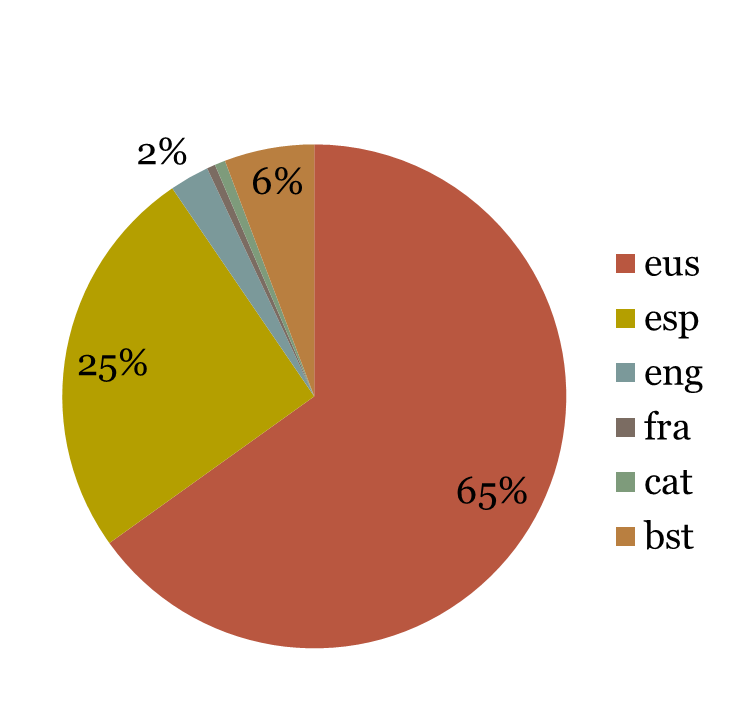
\includegraphics[width=\linewidth]{txio_heldu}
    \caption{Adult personal tweets.}
  \end{subfigure}
  \begin{subfigure}[b]{0.48\linewidth}
    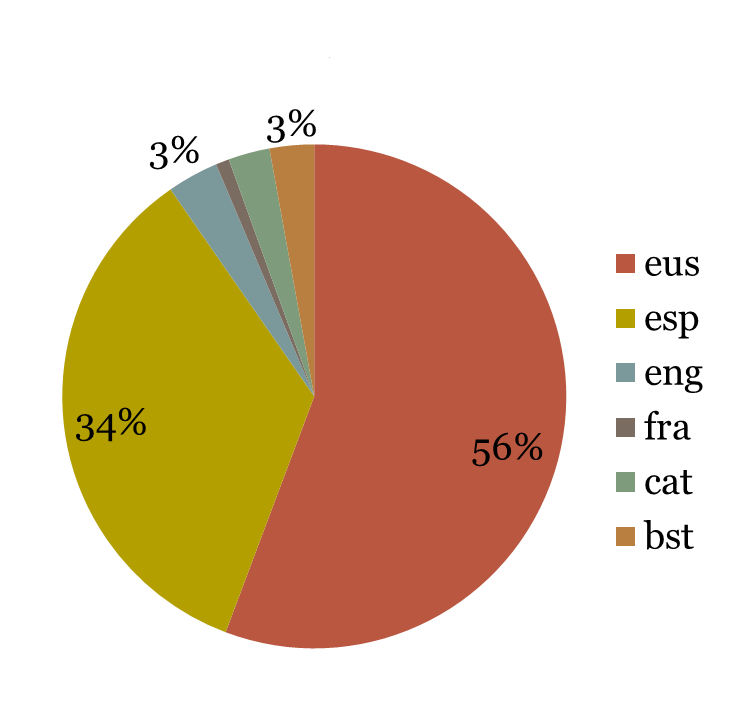
\includegraphics[width=\linewidth]{birtxio_heldu}
    \caption{Adult retweets.}
  \end{subfigure}
  \caption{Adults in the Large Corpus: 5.508 users.}
  \label{fig:adults}
\end{figure}

If we take a look at the tweets written only in Basque, we find that 2.634.534 tweets have been published, containing more than 32M tokens. Figure  \ref{fig:txio luze held} shows their distribution according to their length in tokens. The average tweet contains 12 tokens. Standard deviation with respect to the average is 5.65. Furthermore, median corresponds to 12, mode being 14 token (more than 200K tweets).

\begin{figure}[H]
  \centering
  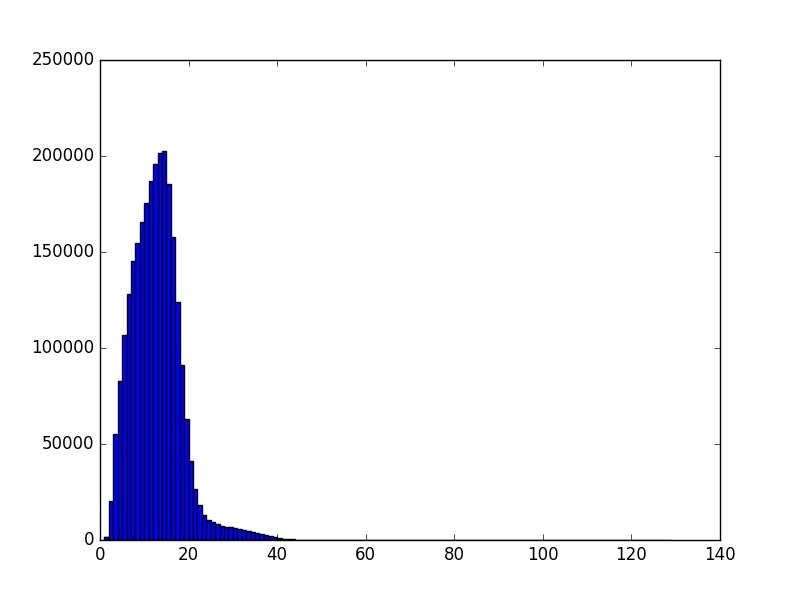
\includegraphics[height=6cm]{graf_for}
  \caption{Distribution of Basque tweets published by adults.}
  \label{fig:txio luze held}
\end{figure}

\subsubsection{Analyzing Young Twitter Users}

The young users corpus contains just one quarter in size with respect to the corpus of adult users. In this case, it can be seen that there are fewer retweets (963.668) than original personal tweets (1.128.124). It is perhaps more noticeable the fact that the use of Basque is less common between young users: 18\% lower for tweets and 24\% lower for retweets. As it is expected, the use of Spanish is higher between young users, reaching 47\% for retweets and 34\% for personal tweets. The data in Figure \ref{fig:gazte txbtx} shows that Basque is less used between young users of Twitter.

\begin{figure}[H]
  \centering
  \begin{subfigure}[b]{0.48\linewidth}
    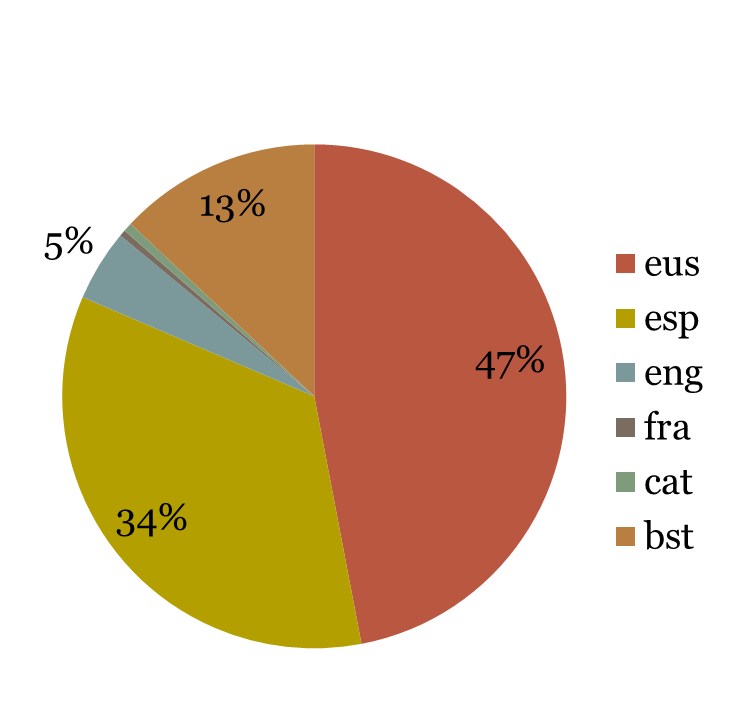
\includegraphics[width=\linewidth]{txio_gazte}
    \caption{Young personal tweets.}
  \end{subfigure}
  \begin{subfigure}[b]{0.48\linewidth}
    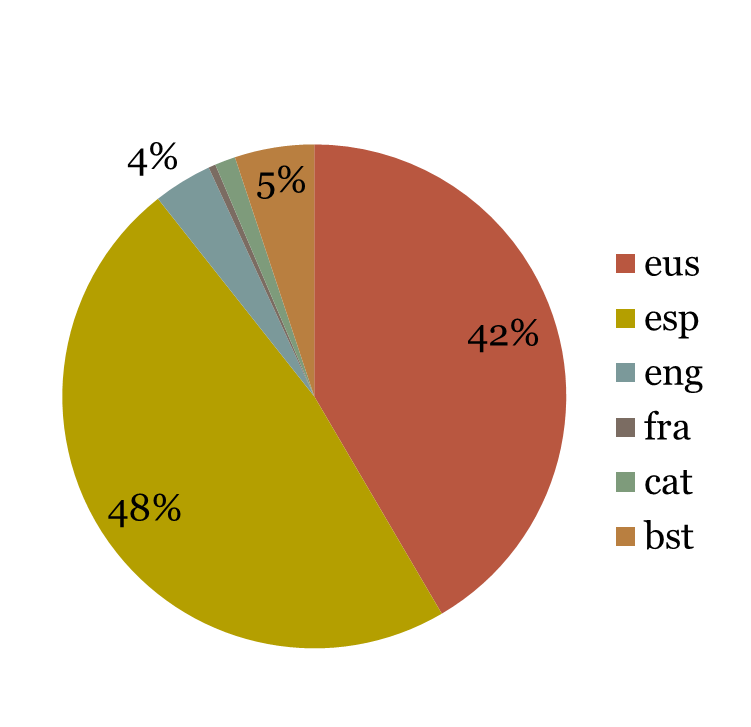
\includegraphics[width=\linewidth]{birtxio_gazte}
    \caption{Young retweets.}
  \end{subfigure}
  \caption{Young users in Large Corpus: 1.579 users.}
  \label{fig:gazte txbtx}
\end{figure}

If we take a look at the tweets written only in Basque, we find that 530.226 personal tweets have been published, containing more than 5M tokens. Figure  \ref{fig:txio luze gzt} shows their distribution according to their length in tokens. The average tweet contains 9 tokens, whereas the standard deviation with respect to the average is 5.49. Furthermore, median corresponds to 8, mode being 6 token (around 45K tweets). In general, it is noticeable the fact that young users published much shorter tweets than adults.

\begin{figure}[H]
  \centering
  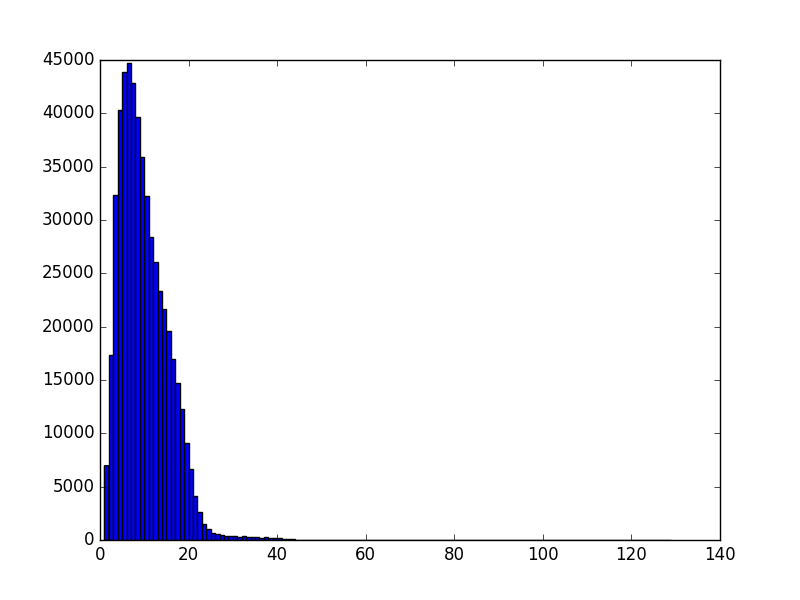
\includegraphics[height=6cm]{graf_inf}
  \caption{Distribution of Basque tweets published by young users.}
  \label{fig:txio luze gzt}
\end{figure}


% ################################################
% ################     TOPICS     ################   
% ################################################

\section{Topics}\label{sec:topics}

The aim of this section is to detect the most frequent topics of Basque tweeters. For this, more than 3 million personal tweets in Basque have been used, separating adults and young in different groups. On the one hand, 2,634,534 personal tweets will be used to predict adult topics and, on the other hand, 530,226 personal tweets will be used to clarify the topics of young people. In this way, from these unstructured data, the topics of the Basque tweeters will be inferred, using the technique of \textit{topic modeling}, applying the algorithm \textit{Latent Dirichlet Allocation} (LDA). Finally, the topics of young and adult speakers will be found out and a comparison will be made between the two groups.


\subsection{\textit{Topic modeling} using LDA}
\label{sec:datu analisi}

The main purpose of this section is to identify the topics of Basque speakers through the LDA algorithm. \textit{Topic modeling} is a commonly used tool in the field of text mining. With this technique, words are grouped according to context, creating more general content with similar words. In this way, the related words will be grouped together, allowing to identify general topics. Thanks to the grouping of words, it will be identified what subjects Basque speakers talk about in the network. The LDA technique will be used to apply topic modeling, creating general topics using words with the same context.

\textit{Latent Dirichlet Allocation} \citep{blei2003latent} makes it possible to classify events that are observable in latent or hidden clusters. This classification occurs thanks to the many hidden features, such as the similarity of words. By linking words and documents, hidden relationships will emerge, in general categories or topics. The LDA is based on the context to classify, the grouping of a word will be based on the words that surround it, regardless of the order of the words. In addition, this groups of words of the same context will share a similar semantic meaning, which will help to define them.

As the first step to complete this action, it will be structuring the documents. The special structure of Tweets makes it difficult for the LDA to be applied properly because these are too short documents and it makes it difficult to find similarities. Taking into account the short nature of the tweets, a special structuring will be carried out to allow a successful topic modeling. The tweets will be grouped by users, in other words, each document will be composed of each person's personal tweets. In this way, to apply the LDA algorithm in a correct way, each document will consist on all the tweets generated by each user \citep{hong2010empirical, zhao2011comparing}. Additionally, to reduce the number of terms and to homogenize the information, words have been lemmatized using the lemmatizer in Basque inside \textit{IXA pipes} program \citep{agerri2014ixa}. 

When LDA is applied, the amount of topics to be identified must be determined, since the algorithm works in this way. With the intention of choosing the correct amount of topics for each model (young and adult), there have been tests with different amounts of topics. It must be said that there is no 'correct' number of topics \citep{binkley2014understanding}, but it should be clear that this number will affect the interpretation of the model \citep{steyvers2007probabilistic}. The amount of topics used is based on the cluster dispersion and in the interpretability. On the one hand, in terms of interpretability, the model is intended to be coherent with social reality, that is, to have a connection with the issues that can be found in Basque society. On the other hand, in terms of dispersion of groups, the intention is to achieve the most dispersed model possible, to find the least possible overlap between groups, since the distance between the groups indicates the conceptual difference of the topics. So, depending on the model (young/adult), an amount of topics have been selected, as more documents are available, more topics can be selected because there is more information. Therefore, the \textit{young} model has fewer topics because the amount of information is smaller. Thus, after completing a comparison between the number of topics for each model, it has been decided to use 20 topics for \textit{adults} model and 12 topics for \textit{young} model. \\

\subsection{Results}
\label{sec:emaitz analisi}
Once the LDA has been completed, the result are displayed by the method \textit{LDAvis} \citep{sievert2014ldavis}, allowing an easy interpretation of each topic. The identity of the topic will be determined by its internal words, \citep{binkley2014understanding}, which will allow to clarify the usual topics spoken by Basque tweeters. Topics have been defined individually for adults (\ref{tab:adult-tp} table) and young people (\ref{tab:young-tp} table), by taking into account the relevant words of each topic.

\begin{table}[H]
  \centering
  \begin{tabular}{|l|l|l|}
    \hline
    \textbf{Topics of adult people} &  \textbf{Representative words in the topic} & \textbf{\% of words} \\ \hline
                   1  Conversation & entzun, iruditu, bizitza, pentsatu, pasatu & 10,5 \%  \\ \hline
                   & listen, imagine, life, think, pass & \\ \hline
                   2  Politics & Euskal Herri, espainia, politiko, estatu, eskubide & 10 \%  \\ \hline
                   & Basque Country, Spain, politics, states, rights & \\ \hline
                   3  Basque tweeters & @txargain, @berria, @boligorria, euskara, idatzi & 6,9 \%  \\ \hline
                   & @user, @newspaper, @user, Basque, write & \\ \hline
                   4  Cultural offer & lehiaketa, sarrera, ikastaro, erakusketa, antzerki & 6,4 \%  \\ \hline
                   & competition, entry, course, exhibition, theater & \\ \hline
                   5  Public administration & udal, zerbitzu, publiko, aurrekontu, euskadi & 6,1 \%  \\ \hline
                   & municipal, services, public, budget, euskadi & \\ \hline
                   6  Basque television & @euskaltelebista, urhanditan, @xabiermadariaga, herritxiki & 5,3 \%  \\ \hline
                   & @television, TV program, @journalist, TV program & \\ \hline
                   7  Tournaments & txapelketa, final, kirol, jokatu, kanporaketa & 5 \%  \\ \hline
                   & championship, final, sports, play, playoffs & \\ \hline
                   8  Basque prisoners & preso, herri, espetxe, iheslari, elkartasun & 4,9 \%  \\ \hline
                   & prisoner, people, prison, fugitive, solidarity & \\ \hline
                   9  Culture & liburu, literatura, filma, poesia, dokumental & 4,8 \%  \\ \hline
                   & books, literature, film, poetry, documentary & \\ \hline
                   10 Social movements & feminista, asanblada, gaztetxe, borroka, langile & 4,8 \%  \\ \hline
                   & feminist, assembly, squatted house, fight, worker & \\ \hline
                   11 Education & ikasle, hezkuntza, irakasle, ikastola, ikastetxe & 4,3 \%  \\ \hline
                   & students, education, teachers, Basque colleges, schools & \\ \hline
                   12 Science & euskara, artikulu, interesgarri, zientzia, teknologia & 4,1 \%  \\ \hline
                   &  Basque, articles, interesting, science, technology& \\ \hline
                   13 Music & kontzertu, disko, talde, entzun, musika & 3,9 \%  \\ \hline
                   & concert, disc, group, listen, music & \\ \hline
                   14 Basque language & euskara, hizkuntza, euskaldun, euskal, ikasi & 3,8 \%  \\ \hline
                   & Basque language, language, Basque speaker, Basque, learn & \\ \hline
                   15 Sports & talde, real, partida, irabazi, jokatu & 3,8 \%  \\ \hline
                   & team, real, match, win, play & \\ \hline
                   16 Gipuzkoa & tolosa, andoain, hernani, ordizi, beasain & 3,7 \%  \\ \hline
                   17 Media in Basque & @berria, @euskalirratia, @argia, @zebrabidea, @iehkohitza & 3,5 \%  \\ \hline
                   18 Donostia & donostia, @donostiakoudala, ezagutu, gipuzkoa & 3,5 \%  \\ \hline
                   19 Nafarroa & nafarroa, baztan, altsasu, irunerri, irun & 2,7 \%  \\ \hline
                   20 Bizkaia & larrabetzu, lekeitio, durango, bermeo, arrasate & 2,6 \%  \\ \hline
  \end{tabular}
  \caption{Topics of adult people}
  \label{tab:adult-tp}
\end{table}


\begin{table}[H]
  \centering
  \begin{tabular}{|l|l|l|}
    \hline
    \textbf{Topics of young people} &  \textbf{Representative words in the topic} & \textbf{\% of words} \\ \hline
                   1  Gipuzkera dialect (informal chat) & in, ne, oain, atxalde, biyar & 14,7 \%  \\ \hline
                   & do, mine, now, late, tomorrow & \\ \hline
                   2  Express feelings & maite, amets, gau, bizi, bihotz & 11,4 \%  \\ \hline
                   & love, dream, night, live, heart & \\ \hline
                   3  Bizkaiera dialect (informal chat) & dau, be, ein, dot, emun, bixar & 10,8 \%  \\ \hline
                   & is, also, do, have, give, tomorrow & \\ \hline
                   4  Sports & partidu, irabazi, jokatu, txapeldun, etapa & 9,9 \%  \\ \hline
                   & match, win, play, champion, stage & \\ \hline
                   5  Cultural activities & areto, antzoki, gaztetxe, tailer, kontzertu & 9,7 \%  \\ \hline
                   & halls, theaters, youth clubs, workshops, concerts & \\ \hline
                   6  To congratulate & zorion, pasatu, animo, eskerrikasko, polit & 9,3 \%  \\ \hline
                   & congratulations, pass, courage, thank you, nice & \\ \hline
                   7  Tell the life & jajaja, bihar, ohera, partido, ikasi & 7,6 \%  \\ \hline
                   & Hahaha, morning, to bed, party, study & \\ \hline
                   8  Bizkaiera dialect (formal chat) & dot, dau, barri, barik, be & 7,1 \%  \\ \hline
                   & have, is, new, without, too & \\ \hline
                   9  Gipuzkera dialect (formal chat) & det, ne, hoi, iruditu, irakurri  & 7,1 \%  \\ \hline
                   & do, mine, that, seem, read & \\ \hline
                   10 Basque prisoners & herri, euskal, etxe, preso, gazte & 6,4 \%  \\ \hline
                   & people, Basque, house, prisoner, youth & \\ \hline
                   11 Athletic CB & aupa, athletic, @athletic, san mames, bilbo  & 3,3 \%  \\ \hline
                   12 Rowing & sailkapen, jardunaldi, maila, txapelketa, estropada & 2,7 \%  \\ \hline
                   & classification, event, level, championship, regatta & \\ \hline
  \end{tabular}
  \caption{Topics of young people}
  \label{tab:young-tp}
\end{table}

By focusing on adults (table \ref{tab:adult-tp}), it can be seen that they use Basque in social networks, especially to deal with issues of a political (politics, Basque prisoners and social movements) or a social (culture, education and Basque language) nature. It should be noted that public political institutions also have their place in this social network (public administration and different administrations from Gipuzkoa, Bizkaia or Nafarroa). It can be considered that talking about social issues is a characteristic for adults, since the topics of social interest have a leading role in this group.

The most common topics of young people (table \ref{tab:young-tp}) are related to their everyday affairs (chat, express feelings, to congratulate and telling life). In some cases, they talk about everyday things, but using their own dialect (Gipuzkera and Bizkaiera). In addition, we can not ignore that sports (sports, Athletic CB, rowing) are also a recurring theme among young people. Focusing on young people, it must be said that they use Basque in social networks, especially in their daily lives to communicate with others.

Comparing the two different age groups, it should be noted that young people use this network for day-to-day things (chat, express feelings, congratulate, tell the life...). It can be said that this social network is used by young people to communicate with their closest. On the other hand, adults use the network to talk about social issues (politics, media, Basque, social movements...). It seems that adults use this social network to socialize messages, especially messages with a political nature. To sum up, it can be said that while the themes of young people and adults are different, the shared functions consist on communication and in the immediate exchange of information.

% ################################################
% ################    RELATIONS   ################   
% ################################################

\section{Relations}\label{sec:connections}

The aim of this section is to study the relationship of Basque tweeters. For this, nearly 3 million retweets in Basque have been used, separating adults and young in different groups. On the one hand, 2,421,058 retweets will be used to predict adult relations and, on the other hand, 400,448 retweets will be used to clarify the relations of young people. In this way, relations of the Basque tweeters will be inferred, using the sender and receiver information of each retweet to build a network of relationships. Finally, the relations of young and adult speakers will be shown and a comparison will be made between the two groups.

\subsection{Relationships graph based on retweets} 
\label{sec:sis harr}

In order to see how the Basque youth and adult are related, a giant graph of each one has been created, based on the content that this groups exchange. To build the graph, two features from each retweet have been used, who retweets and who has been retweeted. In this way, the data source will be the source and the target of each retweet. Based on these two characteristics, two graphs have been created using the \textit{gephi} program \citep{bastian2009gephi}.

Once the graphs have been created, the first step will be to divide each subgroup, using the modularity algorithm \citep{blondel2008fast}. The second step will be to give the network a spatial structure by using the \textit{ForceAtlas2} algorithm \citep{jacomy2014forceatlas2}, ordering the nodes according to the community to which they belong. Finally, the identity of each subgroup or community has been defined, using the most important nodes in these subgroups. In this way, it can be seen how the communities of each graph are structured, on the one hand the 33,277 nodes of the adults, and on the other hand, the 24,987 nodes of the young people .

\subsection{Results}
\label{sec:emaitz analisi harr}

After creating two independent graphs with the youth and adult data, each network was split into subgroups to see how the groups are formed. Then, the subgroups will be defined, based on the most important nodes of each one. With this, the relations of the Basque speakers community of Twitter can be shown.

If we observe the subgroups derived from the graph of \textbf{adults} (table \ref{tab:tab harr hld}), we can see that they have a common characteristic, since all the groups have a relationship with the Basque Country. It can be seen, that in the case of adult people, Basque language is used to talk about Basque issues, highlighting politics (Nationalist left) and current affairs (news). In this way we can say that the function of Twitter is the usual (politics and current affairs), but the focus is on the Basque community itself.

\begin{itemize}
\item \textit{Nationalist Left} (27,92 \%): This subgroup is made up of nodes with a specific political orientation, specifically for the members of the Nationalist Left. In addition to the users that appear in the first column of the table \ref{tab:tab harr hld}, there are also many important nodes that are people (@ArnaldoOtegi, @jpermach, @JosebaAlvarez...) or institutions (@sortuEH, @LAB...) of the Nationalist Left. This is the main group, joined by more than a quarter of all nodes that corresponds to the relationship of a certain political orientation.
\end{itemize}

\begin{itemize}
\item \textit{News} (23,77 \%): This group, related to news, will be formed by almost a quarter of all users. Most of the nodes of this subgroup are related to the media, specially several users related to the EITB (Basque public television) team. 
\end{itemize}

\begin{itemize}
\item \textit{Basque language} (15,34 \%): In the 3rd subgroup, there are subjects related to the Basque language, such as media in Basque (@zuzeu, @Gaztezulo, @ArabakoALEA), associations for the promotion of Basque (@AEK\_eus, @EHEbizi...) as well as several individuals related to Basque (@KikeAmonarriz, @KoldoTellitu, @MertxeMugika).
\end{itemize}

\begin{itemize}
\item \textit{Music and GED} (13,56 \%): In the fourth subgroup, there is a special phenomenon, since it brings together two different groups in the same subgroup. The first part would be about music, since there are different users related to the music scene (@EsneBeltza, @ZuriHidalgo, @ZeEsatek, @40minuturock, @hesiantaldea, @ItzrrSemeak ...). The second part would be related to the users of the Gure Esku Dago dynamic (@GoierrikoGED, @GEDTolosaldea, @GureEskuDagoDon ...), this dynamic could be considered as the Basque sovereignty Movement.
\end{itemize}

\begin{itemize}
\item \textit{Basque tweeters} (13,10 \%): In this last subgroup, we would have common Basque users, being important subjects of the Basque community. It would be a group of well-known individuals, usually followed by the Basque community.
\end{itemize}

\begin{table}[H]
  \centering
  \begin{tabular}{|l|l|l|l|l|}
    \hline
    \textbf{Nationalist left}  &  \textbf{News} &  \textbf{Basque language} &  \textbf{Music and GED} &  \textbf{Basque tweeters}\\ \hline 
    @naiz\_info &  @berria &  @zuzeu &  @XMadariagaI &  @boligorria\\ \hline
    @HamaikaTb &  @eitbAlbisteak &  @KikeAmonarriz &  @gaizkapenafiel &  @zaldieroa\\ \hline
    @larbelaitz & @euskaltelebista &  @Sustatu &  @JGGarai &  @urtziurkizu\\ \hline
    @topatu\_eus &  @euskadi\_irratia &  @Gaztezulo &  @EsneBeltza & @landergarro \\ \hline    
    @axierL & @tolosaldeataria & @AEK\_eus  & @UrHanditan  &  @ielortza\\ \hline
  \end{tabular}
  \caption{Most important nodes for the subgroups of adult people.}
  \label{tab:tab harr hld}
\end{table}

Regarding to \textbf{young} people's graph subgroups (table \ref{tab:tab harr gzt}), it can be seen that there are similarities and differences with the adult graph. Focusing on the similarities, it can be seen that \textit{Basque language}, \textit{Nationalist left} and \textit{News} are important subgroups in both graphs. These common subgroups can be related to politics and immediacy, which are the basic characteristics of Twitter identity. On the other hand, taking into account the differences, it should be noted that groups related to leisure also take a central stage, such as \textit {Sports} and \textit{Music}. To finish, it is worth pointing out that in this case young Basque speakers also take Twitter as a channel to comment on everyday life, in which case the different subgroups are related to close events.

\begin{itemize}
\item \textit{Sports} (21,61 \%): This subgroup, which includes most of the nodes of the youth model, is related to sports. The group would be made up of sports teams or organizations (@RealSociety, @RealSociedadEUS, @ASPEpelota, @SDEibar ...), as well as its athletes (@InigoMartinez, @AmetsTxurruka, @XabierUsabiaga, @Markelirizar ...). However, the most important nodes are sports journalists (@iBROKI, @XabierEuzkitze, @Imagreto, @bzarrabeitia, @TxetxuUbieta...) and the media (@berria, @euskaltelebista, @eitbkirolak, @euskadi\_irratia...). Once again, it can be clearly seen that, despite being the subgroup of sports, the media are the real protagonists.
\end{itemize}

\begin{itemize}
\item \textit{Basque language} (20,70 \%): In this second subgroup, we would have a fifth of all the nodes, being a large group. In this case, the most important nodes are related to the Basque language (@EsaldiakEuskara, @euskarazEH, @Bertsotan, @bertsolaritza, @Euskeraz\_Bizi ...). In subgroups of adults, a community related to this topic has also been found, although the nodes are different, the topic coincides.
\end{itemize}

\begin{itemize}
\item \textit{Nationalist left} (17,12 \%): This third group would be composed of nodes related to the nationalist left. For example, media (@naiz\_info, @topatu\_eus, @inform7irratia, @naizplus...), organizations (@ernaigazte, @ehbildu, @sortuEH...) and individuals (@ArnaldoOtegi, @lauramintegi...) related to the nationalist left. Once again, it can be seen that there are similarities with subgroups of adults, very similar in this particular case both in the topic and in the nodes.
\end{itemize}

\begin{itemize}
\item \textit{News} (14,92 \%): In the fourth subgroup, it can be seen that the most important nodes correspond to Basque media (@argia, @HamaikaTb, @eitb Albums, @zuzeu, @Gaztezulo). Once again, It can be seen that there are some similarities between young people and adults.
\end{itemize}

\begin{itemize}
\item \textit{Music} (11,35 \%): In the final subgroup, although it is quite diverse, it can be said that the most important nodes are related to music. Among these, the media that talk about music (@gaztea, @DidaGaztea), music groups (@berritxarrak, @muguruzafm, @Glaukomaband), as well as some record companies (@BagaBigaeus).
\end{itemize}

\begin{table}[H]
  \centering
  \begin{tabular}{|l|l|l|l|l|}
    \hline
    \textbf{Sports}  &  \textbf{Basque language} &  \textbf{Nationalist left} &  \textbf{News} &  \textbf{Music}\\ \hline 
     @berria &  @enekogara & @naiz\_info  &  @argia &  @berritxarrak\\ \hline
     @euskaltelebista & @GureEskuDago  & @larbelaitz  &  @HamaikaTb &  @gaztea\\ \hline
     @iBROKI &  @EsaldiakEuskara &  @topatu\_eus &  @eitbAlbisteak &  @izanpirata\\ \hline
     @RealSociedad & @ZuriHidalgo  & @ArnaldoOtegi  & @MaddalenIriarte  &  @eitbeus\\ \hline
     @XabierEuzkitze &  @MeriLing1 & @ernaigazte  &  @ielortza &  @LeakoHitza\\ \hline
  \end{tabular}
  \caption{Most important nodes for the subgroups of young people.}
  \label{tab:tab harr gzt}
\end{table}

Once the subgroups of both models have been interpreted and defined, a comparison between the two has been done. It can be seen (table \ref{tab:taldeak}), both adults and young people, even though they have different preferences in their relationship, they have a common part. On the one hand, the political nature and immediacy of this social network would be a common part, even if it is more noticeable for adults. Additionally, it should be pointed out that in most subgroups, media-related users play an important role, confirming the informative nature of Twitter. On the other hand, we must emphasize that Basque users use Basque language, especially to talk about events or topics around them, linked to the context of the Basque Country. To conclude, it must be said that the community of Basque tweeters, apart from sharing the general characteristics of Twitter (immediacy and political character), has its own peculiarity, to use Basque language to speak about Basque topics.

\begin{table}[H]
           \centering
           \captionsetup[subtable]{position = below}
          \captionsetup[table]{position=top}
           
           \begin{subtable}{0.45\linewidth}
               \centering
               \begin{tabular}{|l|c|}
                   \hline
                   \textbf{Adult people subgroups} & \textbf{Number of nodes} \\ \hline
                   Nationalist left & 27,92 \% \\ \hline
                   News & 23,77 \% \\ \hline
                   Basque language & 15,34 \% \\ \hline
                   Music and GED & 13,56 \% \\ \hline
                   Basque tweeters & 13,10 \% \\ \hline
               \end{tabular}
               \caption{Relationship communities of adult people.}
               \label{tab:heldu talde}
           \end{subtable}%
           \hspace*{4em}
           \begin{subtable}{0.45\linewidth}
               \centering
               \begin{tabular}{|l|c|}
                   \hline
                   \textbf{Young people subgroups} & \textbf{Number of nodes} \\ \hline
                   Sports & 21,61 \% \\ \hline
                   Basque language & 20,70 \% \\ \hline
                   Nationalist left & 17,12 \% \\ \hline
                   News & 14,92 \% \\ \hline 
                   Music & 11,35 \% \\ \hline
               \end{tabular}
                \caption{Relationship communities of young people.}
                 \label{tab:gazte talde}
           \end{subtable}
           \caption{Relationship communities in each model.}
           \label{tab:taldeak}
       \end{table}


% ####################################################
% ################     CONCLUSION     ################   
% ####################################################


\section{Conclusion and Future Work}
\label{sec:conclusion}

We have shown how to develop 

Twitter sare sozialera konektatuta dauden euskal hiztun gazteen on-line errealitatera hurbilpen bat egitea lortu da. Helburu orokor hori betetzeko hainbat pausu eman dira, lehenik eta behin Twitter sare sozialetik euskal erabiltzaileen datu kantitate erraldoiak erauzi dira. Bigarrenik, erauzitako euskal txiolariak sailkatu dira gazte eta heldu artean, gazteen errealitatea ezagutzea baita helburu nagusia. Hirugarrenik eta azkenik, gazte eta helduen gaiak zeintzuk diren eta harremanak nola ematen diren argitu da, bi talde ezberdinen errealitatea zein den erakutsiz. Lan honekin, frogatuta geratzen da gizarte-zientzia eta konputazio-zientzien arteko konbinaketa aberasgarria dela, Hizkuntzaren Prozesamenduko teknikak aplikatuz, ezaugarri demografikoak iradoki edota diskurtso analisia bezalako atazak burutu daitezkeela erakutsi delarik.\\
\indent Datuen erauzketaren inguruko balorazioa burutzerakoan, esan daiteke datu-iturri berri bat ireki dela Twitterreko informazioa erauzteko garatutako teknikari esker. Erauzketa teknika honi esker, datu kantitate handiak (Big Data) lortu dira oso kostu txikiarekin. Horrez gain, gazteen ingurunera hurbiltzea lortu da, hauen errealitatea hobeto ezagutzeko lehenengo pausua emanez. Hala ere, datu-iturri berri honek ere baditu bere mugak, Twitterreko erabiltzaileengan mugatzen dela ikerketa. Hobekuntza moduan, datu-iturri berriak gehitu daitezke beste sare sozial batzuen erauzketa burutuz, adibidez Instagram, Snaptchat edota Facebook erauziz, edukia publiko jarriko balute. Baina, teknika honekin sare sozialen erabiltzaileen informazioa soilik lortuko litzateke eta, gaur egun behintzat, populazioaren zati handi bat kanpo geratuko litzateke. Horrez gain ere, Twitterrek berak jarritako mugak (erabiltzaileko 3200 txio gehienez jota eta 15 erabiltzaile bakarrik 15 minuturo) ere kontutan hartu behar dira, lana dezente mantsotu egiten baitute muga horiek. Datu-iturri berri honen mugak alde batera utzita, sistema arrakastatsu bat garatu dela onartu beharra dago, ia 8.000 euskal erabiltzaile erauztea lortu baitira, 10 milioi txio baino gehiago geureganatuz.\\
\indent Ikerketa lan honen atal garrantzitsuetako bat gazteak eta helduak ezberdintzean oinarritu da, interesetako bat gazteen errealitatea ezagutzea izanik. Gazte/heldu ezberdintzea adinaren arabera burutu ordez, testuaren formaltasunaren arabera burutu da, adinaren araberako etiketatzeak kostu altuegia baitzuen. Hortaz, adinaren etiketatzearen zailtasunen aurrean, lasterbide metodologikoa erabiltzea erabaki da, testu informalaren kontzentrazioa altua bada gaztea izango dela erabakiz. Honela, txioen corpus txiki bat etiketatu ostean, sailkapena burutu da \textit{IXA pipes} dokumentu sailkatzailea erabiliz erabiltzaile bakoitzaren testuaren formaltasunean oinarrituta. Sistema honek, emaitza fidagarriak lortzeaz gain, etiketatutako corpus txikiekin ere sailkapena ondo egiten duela esan beharra dago. Etorkizunerako, egokia izango litzateke sailkapena adinaren arabera burutzea, horretarako corpus berri bat etiketatu beharko litzatekeela argi edukiz. Hala ere, \textit{IXA pipes} dokumentu sailkatzaileari esker, etiketatutako corpus txikiekin ere sailkapen egokiak burutu daitezke, sistema hornitzen duten egiturarik gabeko datu multzoetan oinarritutako hitzen irudikapenei esker. Etiketatutako corpus txikiekin ere ondo sailkatzen duen sistema bati esker, ikertzaile txikiek aukera gehiago daukate atazak modu arrakastatsuan garatzeko, corpus handiak etiketatzea lan eta kostu handia baitira.\\
\indent Behin gazte eta helduen taldeak ezberdinduta daudelarik, hauen gai ohikoenak zeintzuk diren azaleratu eta hauen harremantzeko modua zein den argitu da hein batean. Lehenik eta behin, euskal erabiltzaileek ze gairi buruz aritzen diren argituko da, horretarako txio pertsonalen testuetan LDA teknika aplikatzean oinarritu garelarik. Gazteek gehienbat, beren gertukoekin komunikatzeko erabiltzen dute sare sozial hau, egunerokotasuneko gertakariak adieraziz. Helduen artean ostera, mezuak gizarteratzeko lanabes modura kontsideratzen dela ikusi daiteke, batez ere izaera politikoa daukaten gaiak plazaratzeko, gizartean pil-pilean dauden gaiei buruz arituz. Gazte eta helduen tematikak ezberdinak izan arren, komunikatzeko eta informazio-trukerako lanabes moduan erabilia da sare sozial hau. Bigarrenik, harremanak nola ematen diren azaleratu da, horretarako euskarazko birtxioetan oinarrituta harreman sare bat sortu delarik. Honez gain, aipatu beharra dago, komunikabideekin erlazionatutako erabiltzaileek garrantzizko papera jokatzen dutela, Twitterren izaera informatiboa konfirmatzen delarik. Erabiltzaile euskaldunek euskara erabiltzen dute, batez ere, beren inguruko gertakari edo gaien inguruan hitz egiteko, gaien arabera ere harreman-taldeak sortuz. Harremanak komunitate konkretuen baitan ematen da eta Euskal Herriko testuinguruarekin erlazionatuta daudela esan daiteke. Ondorioztatu daiteke, euskara, euskaldunen gaiei buruz hitz egiteko erabiltzen dela gehienbat.\\
\indent Lan honen galdera nagusiari erantzuteko asmoarekin, euskaraz aritzen diren gazteak zertaz aritzen diren eta zeinekin harremantzen diren argitzen saiatu gara. Sarritan ezezaguna den gazteen errealitateari hurbilpen honekin, etorkizuna izango diren gazteen euskararekiko portaera ikusi ahal izango da. Gazteak euskaraz hitz egitera bultzatzen dituen gaiak eta harremantzeko moduak azaleratzea izango da asmoa, gazteak euskaraz hitz egitera animatzen dituzten zergatiak argituz. Gazteak eguneroko bizitzari eta kirolei buruz aritzen dira gehienbat, honek erakusten du, beren gertukoekin komunikatzeko erabiltzen dutela sare sozial hau, egunerokotasuneko gertakariak adieraziz. Harremanei begira, euskal erabiltzaileak intereseko gaien arabera harremantzen direla ikusi da, gazteen harremanak, euskal herriko gai politikoekin eta aisialdiarekin lotzen direlarik.\\
\indent Lan honek euskara XXI. mendeko testuingurura nola moldatzen ari den ezagutzeko aukera eman du ere, ikusi ahal izan da, euskara presente dagoela sare sozialetan, euskarazko 6 milioi txio baino gehiago lortu baititugu ia 8.000 erabiltzaile ezberdinenak. Euskara sare sozialak bezalako teknologia berrietan presente egoteak esan nahi du, geure hizkuntza erronka berrietara egokitzeko kapaza dela, euskaldunen sorkuntza kapazitateari esker teknologia berrietan ere erabilia delarik. Euskal komunitatearen baitako erakunde eta norbanako erreferentzial gehienak komunikabideekin eta Ezker Abertzalearekin zerikusia daukatela ikusi ahal izan da. Honez gain, erabiltzaile euskaldunek eginiko erabileratik ondorioztatu dezakegu euskara euskaldunen inguruko gaiez aritzeko erabiltzen dela gehienbat. Laburbilduz, esan daiteke, euskara testuinguru berrietara moldatzeko gai dela, betiere hiztunen komunitatearen egunerokotasuneko errealitatearekin modu estuan lotuta. Honek erakusten digu, globalizatutako eta etengabe konektatutako mundu honetan ere, euskaldunek badutela gaitasun berezi bat beren lekua bilatu eta bertan finkatzeko.\\ 


%%%%%%%%%%%%%%%%%%%%%%%%%%%%%%%%%%%%%%%%%%


\section{Patents}
This section is not mandatory, but may be added if there are patents resulting from the work reported in this manuscript.

%%%%%%%%%%%%%%%%%%%%%%%%%%%%%%%%%%%%%%%%%%
\vspace{6pt} 

%%%%%%%%%%%%%%%%%%%%%%%%%%%%%%%%%%%%%%%%%%
%% optional
%\supplementary{The following are available online at \linksupplementary{s1}, Figure S1: title, Table S1: title, Video S1: title.}

% Only for the journal Methods and Protocols:
% If you wish to submit a video article, please do so with any other supplementary material.
% \supplementary{The following are available at \linksupplementary{s1}, Figure S1: title, Table S1: title, Video S1: title. A supporting video article is available at doi: link.}

%%%%%%%%%%%%%%%%%%%%%%%%%%%%%%%%%%%%%%%%%%
\authorcontributions{For research articles with several authors, a short paragraph specifying their individual contributions must be provided. The following statements should be used “conceptualization, X.X. and Y.Y.; methodology, X.X.; software, X.X.; validation, X.X., Y.Y. and Z.Z.; formal analysis, X.X.; investigation, X.X.; resources, X.X.; data curation, X.X.; writing—original draft preparation, X.X.; writing—review and editing, X.X.; visualization, X.X.; supervision, X.X.; project administration, X.X.; funding acquisition, Y.Y.”, please turn to the  \href{http://img.mdpi.org/data/contributor-role-instruction.pdf}{CRediT taxonomy} for the term explanation. Authorship must be limited to those who have contributed substantially to the work reported.}

%%%%%%%%%%%%%%%%%%%%%%%%%%%%%%%%%%%%%%%%%%
\funding{Please add: ``This research received no external funding'' or ``This research was funded by NAME OF FUNDER grant number XXX.'' and  and ``The APC was funded by XXX''. Check carefully that the details given are accurate and use the standard spelling of funding agency names at \url{https://search.crossref.org/funding}, any errors may affect your future funding.}

%%%%%%%%%%%%%%%%%%%%%%%%%%%%%%%%%%%%%%%%%%
\acknowledgments{In this section you can acknowledge any support given which is not covered by the author contribution or funding sections. This may include administrative and technical support, or donations in kind (e.g., materials used for experiments).}

%%%%%%%%%%%%%%%%%%%%%%%%%%%%%%%%%%%%%%%%%%
\conflictsofinterest{Declare conflicts of interest or state ``The authors declare no conflict of interest.'' Authors must identify and declare any personal circumstances or interest that may be perceived as inappropriately influencing the representation or interpretation of reported research results. Any role of the funders in the design of the study; in the collection, analyses or interpretation of data; in the writing of the manuscript, or in the decision to publish the results must be declared in this section. If there is no role, please state ``The funders had no role in the design of the study; in the collection, analyses, or interpretation of data; in the writing of the manuscript, or in the decision to publish the results''.} 

%%%%%%%%%%%%%%%%%%%%%%%%%%%%%%%%%%%%%%%%%%
%% optional
\abbreviations{The following abbreviations are used in this manuscript:\\

\noindent 
\begin{tabular}{@{}ll}
MDPI & Multidisciplinary Digital Publishing Institute\\
DOAJ & Directory of open access journals\\
TLA & Three letter acronym\\
LD & linear dichroism
\end{tabular}}

%%%%%%%%%%%%%%%%%%%%%%%%%%%%%%%%%%%%%%%%%%
%% optional
\appendixtitles{no} %Leave argument "no" if all appendix headings stay EMPTY (then no dot is printed after "Appendix A"). If the appendix sections contain a heading then change the argument to "yes".
\appendixsections{multiple} %Leave argument "multiple" if there are multiple sections. Then a counter is printed ("Appendix A"). If there is only one appendix section then change the argument to "one" and no counter is printed ("Appendix").
\appendix
\section{}
\unskip
\subsection{}
The appendix is an optional section that can contain details and data supplemental to the main text. For example, explanations of experimental details that would disrupt the flow of the main text, but nonetheless remain crucial to understanding and reproducing the research shown; figures of replicates for experiments of which representative data is shown in the main text can be added here if brief, or as Supplementary data. Mathematical proofs of results not central to the paper can be added as an appendix.

\section{}
All appendix sections must be cited in the main text. In the appendixes, Figures, Tables, etc. should be labeled starting with `A', e.g., Figure A1, Figure A2, etc. 

%%%%%%%%%%%%%%%%%%%%%%%%%%%%%%%%%%%%%%%%%%
% Citations and References in Supplementary files are permitted provided that they also appear in the reference list here. 

%=====================================
% References, variant A: internal bibliography
%=====================================
\reftitle{References}
\externalbibliography{yes}
\bibliography{biblio,/home/ragerri/references/references}


%\begin{thebibliography}{999}
%% Reference 1
%\bibitem[Author1(year)]{ref-journal}
%Author1, T. The title of the cited article. {\em Journal Abbreviation} {\bf 2008}, {\em 10}, 142-149, doi:xxxxx.
%% Reference 2
%\bibitem[Author2(year)]{ref-book}
%Author2, L. The title of the cited contribution. In {\em The Book Title}; Editor1, F., Editor2, A., Eds.; Publishing House: %City, Country, 2007; pp. 32-58, ISBN.
%\end{thebibliography}

%=====================================
% References, variant B: external bibliography
%=====================================
%\externalbibliography{yes}
%\bibliography{your_external_BibTeX_file}

%%%%%%%%%%%%%%%%%%%%%%%%%%%%%%%%%%%%%%%%%%
%% optional
\sampleavailability{Samples of the compounds ...... are available from the authors.}

%% for journal Sci
%\reviewreports{\\
%Reviewer 1 comments and authors’ response\\
%Reviewer 2 comments and authors’ response\\
%Reviewer 3 comments and authors’ response
%}

%%%%%%%%%%%%%%%%%%%%%%%%%%%%%%%%%%%%%%%%%%
\end{document}
